% Bản dịch tiếng Việt của main.tex (để đọc/rà soát). Dịch phần chữ; GIỮ NGUYÊN mọi
% công thức, bảng (\input{tab_*}), hình, trích dẫn (\cite), nhãn (\label/\ref) và SỐ LIỆU.
% Thuật ngữ kỹ thuật giữ tiếng Anh theo quy ước đề tài. Build: pdflatex mainvi && bibtex mainvi && pdflatex mainvi x2.
% CAS loads the legacy STIX fonts. Unicode engines use unicode-math below.
\RequirePackage{iftex}
\ifPDFTeX\else
  \makeatletter
  \disable@package@load{stix}{}
  \makeatother
\fi
\documentclass[a4paper,fleqn]{cas-dc}
\ifPDFTeX
  \usepackage[utf8]{inputenc}
  \usepackage[T5]{fontenc}
\else
  \usepackage{fontspec}
  \usepackage{unicode-math}
  \setmathfont{latinmodern-math.otf}
\fi
\usepackage[numbers,sort&compress]{natbib}
\usepackage{amsmath,amssymb}
\usepackage{booktabs}
\usepackage{tabularx}
\usepackage{array}
\usepackage{enumitem}
\usepackage{microtype}
\usepackage{hyperref}
\usepackage{xurl}
\usepackage{xcolor}
\usepackage{graphicx}
\usepackage{adjustbox}
\usepackage{placeins}
\graphicspath{{figures/}{./}}
\usepackage{tikz}
\usetikzlibrary{arrows.meta,positioning}

% Float: giữ bảng/hình gần chỗ nhắc tới, không đùn về cuối.
\renewcommand{\topfraction}{0.9}
\renewcommand{\bottomfraction}{0.8}
\renewcommand{\textfraction}{0.07}
\renewcommand{\floatpagefraction}{0.8}
\setcounter{topnumber}{3}
\setcounter{bottomnumber}{2}
\setcounter{totalnumber}{5}
\renewcommand{\dbltopfraction}{0.9}
\renewcommand{\dblfloatpagefraction}{0.8}
\setcounter{dbltopnumber}{3}

\newcommand{\Ntau}{N_{\tau}}

\begin{document}
\let\WriteBookmarks\relax
\def\floatpagepagefraction{1}
\def\textpagefraction{.001}
\shorttitle{Tấn công NMS có thực sự làm chậm bộ phát hiện?}
\shortauthors{Pham, Mai và Dinh}
\title[mode=title]{Tấn công cạn kiệt tài nguyên qua NMS có thực sự làm chậm bộ phát hiện? Một nghiên cứu đo lường trên CPU ghim lõi}
\hypersetup{pdftitle={Tan cong can kiet tai nguyen qua NMS co thuc su lam cham bo phat hien? Mot nghien cuu do luong tren CPU ghim loi}}
\author[1]{Pham Tuan Anh}
\author[1]{Mai Quoc Bao}
\author[1]{Dinh Phuong Nam}[orcid=0009-0006-1239-1266]
\cormark[1]
\ead{dp.nam@hutech.edu.vn}
\cortext[1]{Tác giả liên hệ.}
\affiliation[1]{organization={Trường Đại học Công nghệ TP.HCM (HUTECH)},
city={TP. Hồ Chí Minh},country={Việt Nam}}

\begin{abstract}
Tấn công cạn kiệt tài nguyên (resource-exhaustion) trên bộ phát hiện đối tượng tối đa hóa số ứng viên đi vào non-maximum suppression (NMS), $\Ntau$, coi đó như một proxy cho độ trễ. Các đánh giá gần đây cho thấy những tấn công này thường không đạt mức làm chậm như công bố, nhưng không cho biết \emph{khi nào} một sự gia tăng của $\Ntau$ trở thành độ trễ đo được. Chúng tôi trả lời bằng một đối chứng dương (positive control) trong đó $\Ntau$ được đặt chính xác, một sàn nhiễu (noise floor) hiệu chuẩn bằng các lượt A/A trên một lõi CPU được ghim và kiểm chứng, và một mô hình ngân sách không tham số, $R \approx 1+\Delta t_{\mathrm{NMS}}/t_{\mathrm{total}}$: ngưỡng dùng trong bài áp dụng cho tổng thời gian tăng thêm, $\Delta t_{\mathrm{total}} > \mathrm{MDE}\times t_{\mathrm{total}}$. Mức tăng ở NMS là một thành phần của tổng đó. Thứ nhất, tiêm $10^2$ tới $10^4$ ứng viên làm tăng độ trễ NMS với mọi cài đặt và hình học, nhưng với hệ số chênh nhau hơn hai bậc độ lớn, và một cap top-300 loại bỏ phần lớn mức tăng. Thứ hai, trên YOLOv8n ngưỡng toàn trình vào khoảng một trăm ứng viên với vòng lặp pure-PyTorch và hàng nghìn với các kernel thư viện; trên YOLOv5s, các biến thể thích ứng của hai tấn công toàn ảnh làm tăng $\Ntau$ vài trăm lần nhưng thời gian toàn trình chỉ vài phần trăm, và một patch di truyền gray-box (Sponge Patch) không làm tăng $\Ntau$. Thứ ba, $\Ntau$ là proxy yếu: dự đoán thời gian NMS chỉ từ $\Ntau$ sai tới vài lần, và mô hình ngân sách đạt quy tắc đăng ký trước ở một nửa số ô của tấn công thật. Các kết quả phát hiện này đúng trên một lõi CPU laptop được ghim. Trên một Raspberry Pi 3B bị ép về 600~MHz, một mô hình phân đoạn có hậu xử lý tăng theo số phát hiện được giữ lại cho thấy chế độ ngược lại: đầu vào bị tấn công mất thời gian gấp 1.798 lần (bốn luồng) và 1.967 lần (một luồng).
\end{abstract}

\begin{keywords}
tấn công cạn kiệt tài nguyên \sep tấn công độ trễ \sep non-maximum suppression (NMS) \sep đo độ trễ \sep adversarial patch \sep tính sẵn sàng (availability)
\end{keywords}

\maketitle

\section{Giới thiệu}
Tấn công cạn kiệt tài nguyên, còn gọi là tấn công độ trễ hay năng lượng--độ trễ, nhắm vào tính sẵn sàng thay vì tính đúng đắn: đầu vào được chế tạo để kéo dài xử lý mà không nhất thiết đổi nhãn \cite{shumailov2021sponge,nicgslowdown2022}. Với một hệ thống tri giác thời gian thực, mỗi khung hình chậm là một hạn chót có thể bị lỡ. Ở các bộ phát hiện một giai đoạn kiểu YOLO, mặt tấn công tự nhiên là non-maximum suppression (NMS): chi phí của greedy NMS tăng theo số hộp ứng viên vượt ngưỡng điểm, và số đó phụ thuộc nội dung ảnh.

Các tấn công đã công bố như Phantom Sponges, Overload và SlowTrack chế tạo đầu vào để tối đa hóa số ứng viên trước NMS, $\Ntau$, dựa trên giả định rằng $\Ntau$ cao làm bộ phát hiện chậm lại \cite{phantom2023,overload2024,slowtrack2024}. Trong các công trình đó $\Ntau$ vừa là đại lượng được tối ưu vừa là lời giải thích cho mức chậm quan sát được. Tuy nhiên chi phí NMS còn phụ thuộc cài đặt, cách các hộp chồng lấn, và cap top-$k$, và NMS chỉ là một công đoạn của pipeline. EVADE đã benchmark các tấn công độ trễ NMS hiện có trên nhiều phần cứng, định dạng mô hình và lượng tử hóa, và thấy chúng không đạt mức chậm như báo cáo trong cấu hình triển khai \cite{evade2025}. EVADE trả lời \emph{liệu} các tấn công đã công bố có hiệu quả không; nó không giải thích \emph{vì sao} chúng không đạt, cũng không cho biết \emph{khi nào} một $\Ntau$ bị thổi phồng sẽ tạo ra độ trễ đo được. Lời giải thích đó cần một đối chứng dương trong đó $\Ntau$ được đặt chính xác, một sàn nhiễu cho biết mức chậm nhỏ nhất mà phép đo phân giải được, và một mô hình quy đổi ứng viên thành mili giây cho một thiết bị và cài đặt cụ thể. Theo chúng tôi biết, chưa công trình nào cung cấp cả ba.

Chúng tôi bắt đầu bằng việc xây Sponge Patch, một patch gray-box cục bộ chỉ đọc điểm tin cậy trước NMS và được tối ưu bằng giải thuật di truyền để tăng $\Ntau$. Dưới một giao thức có ghim lõi được kiểm chứng và sàn nhiễu đã hiệu chuẩn, patch này không làm tăng $\Ntau$ trên YOLOv8n. Thay vì báo cáo thêm một tấn công nữa, chúng tôi nghiên cứu chính proxy mà cả dòng tấn công này dựa vào: dưới điều kiện nào một sự gia tăng của $\Ntau$ trở thành độ trễ toàn trình, và phải lớn bao nhiêu? Kết quả trung tâm của chúng tôi là một tiêu chí có thể kiểm trước khi chạy bất kỳ tấn công nào: ngưỡng dùng trong bài so mức tăng thời gian toàn trình với $\mathrm{MDE}\times t_{\mathrm{total}}$. Chúng tôi đo các thành phần của tiêu chí này, kiểm nó một cách đón đầu (prospective) trên các biến thể thích ứng của hai tấn công toàn ảnh đã công bố, và dùng nó để giải thích vì sao cả các biến thể đó lẫn Sponge Patch gần như không làm đổi thời gian toàn trình trên CPU. Chúng tôi chia câu hỏi thành bốn câu hỏi con.
\begin{description}[leftmargin=2.5em,labelwidth=2.2em,itemsep=2pt]
\item[Q1] Khi các ứng viên được kiểm soát, độ trễ NMS phụ thuộc $\Ntau$ ra sao trong khoảng $10^2$ tới $10^4$ ứng viên?
\item[Q2] Cài đặt NMS, hình học hộp và cap top-$k$ làm thay đổi sự phụ thuộc đó bao nhiêu?
\item[Q3] Cần bao nhiêu ứng viên để thời gian toàn trình vượt lên trên sàn nhiễu, và các patch thật (YOLOv8n) có đạt mức đó không; với các tấn công toàn ảnh thật (YOLOv5s), mức tăng NMS có vượt ngưỡng tính cho mô hình đó không?
\item[Q4] Một bộ dự đoán chỉ dựa trên $\Ntau$ chính xác đến đâu, cho thời gian NMS và cho thời gian toàn trình?
\end{description}

\paragraph{Đóng góp.}
(i) Một tiêu chí được hiệu chuẩn theo sàn nhiễu cho tấn công cạn kiệt tài nguyên qua NMS: với mô hình ngân sách kiểu Amdahl $R \approx 1 + \Delta t_{\mathrm{NMS}}/t_{\mathrm{total}}$, ngưỡng toàn trình là $\Delta t_{\mathrm{total}} > \mathrm{MDE}\times t_{\mathrm{total}}$. Mô hình ngân sách ước lượng phần đóng góp của NMS khi các công đoạn khác giữ nguyên. (ii) Một bản đồ đối chứng dương từ $\Ntau$ tới độ trễ NMS và độ trễ toàn trình theo cài đặt, hình học hộp và cap top-$k$, kèm các ngưỡng toàn trình $N^{*}$ đo được: cùng một $\Ntau$ có thể tốn nhiều hơn hoặc ít hơn tới hơn hai bậc độ lớn tùy các yếu tố này. (iii) Bằng chứng rằng $\Ntau$ là một proxy yếu ngay cả trên tấn công thật: dự đoán thời gian NMS chỉ từ $\Ntau$ sai tới vài lần, một phần mức chậm đo được nằm ngoài NMS, và mô hình ngân sách đã đăng ký trước đạt ở một nửa số ô tấn công thật. (iv) Một giao thức đo tái sử dụng được: ghim lõi được kiểm chứng dưới tải, đo thời gian từng công đoạn, hiệu chuẩn A/A, đăng ký trước và bảng sinh tự động. (v) Một kiểm chéo toàn trình trên board Arm, Raspberry Pi 3B bị ép về 600~MHz, nơi một pipeline phân đoạn dành gần một nửa thời gian cho hậu xử lý sau tấn công và mức chậm là lớn.

\section{Công trình liên quan}
\label{sec:related}
\paragraph{Tấn công cạn kiệt tài nguyên.}
Tấn công vào tính sẵn sàng coi chi phí tính toán là một bề mặt tấn công bên cạnh tính đúng đắn. Sponge examples làm tăng năng lượng hoặc độ trễ của mạng bằng đầu vào được chế tạo \cite{shumailov2021sponge}, và NICGSlowDown kéo dài chuỗi sinh ra của một mô hình chú thích ảnh \cite{nicgslowdown2022}. Ở bộ phát hiện, nút thắt phụ thuộc nội dung là NMS, có chi phí tăng theo số hộp ứng viên. Phantom Sponges tối ưu một nhiễu toàn ảnh white-box để số hộp vượt ngưỡng bùng nổ \cite{phantom2023}; Overload đi cùng hướng trên thiết bị biên, nơi một lần suy luận dài là đủ để lỡ hạn chót \cite{overload2024}; SlowTrack chuyển mục tiêu sang bộ theo dõi và chuỗi nhận thức của xe tự hành \cite{slowtrack2024}, nên bỏ NMS khỏi bộ phát hiện không loại được mọi chi phí phụ thuộc nội dung. Tấn công độ trễ bằng lật bit dùng một mô hình đe dọa khác, can thiệp vào tham số thay vì đầu vào \cite{bitflip2025}.

\paragraph{Đánh giá và phòng thủ tính sẵn sàng.}
Underload dùng huấn luyện đối kháng chú ý nền để cân bằng độ chính xác trên ảnh sạch và thông lượng thời gian thực; nó bảo vệ dịch vụ trực tiếp nhưng cần quyền truy cập và huấn luyện lại mô hình \cite{underload2025}. EVADE định nghĩa một khung đánh giá, áp dụng cho các tấn công độ trễ NMS hiện có trên nhiều nền tảng phần cứng, định dạng mô hình và thiết lập lượng tử hóa, và báo cáo rằng các tấn công này không tạo ra mức tăng độ trễ như tuyên bố, không chuyển giao sang mô hình khác, và giữ mức tăng trong yêu cầu độ trễ của tác vụ phía sau \cite{evade2025}. Chúng tôi tiếp nhận yêu cầu đo trên thực thi của hướng đánh giá đó nhưng hỏi một câu khác: EVADE đo xem các tấn công cho trước có đạt tuyên bố hay không, còn chúng tôi mô hình hóa và đo khi nào một mức tăng của đại lượng được tối ưu có thể tạo ra độ trễ, độc lập với bất kỳ tấn công cụ thể nào (Bảng~\ref{tab:related}).

\paragraph{Patch đối kháng.}
Dòng patch cục bộ chủ yếu nhắm tới phát hiện sai chứ không phải làm chậm. Các benchmark và phòng thủ tập trung vào đánh giá nhất quán, làm sạch (purification), phát hiện vùng và huấn luyện đối kháng \cite{apde2025,pbcat2025,oddr2025,diffpad2025,unifiedpatchdet2025,antistyler2026,trace2026}; vì một công đoạn thêm vào có thể tự nó làm tăng độ trễ, đánh giá phòng thủ nên báo cáo cả độ chính xác lẫn chi phí hậu xử lý. Các công trình về vị trí đặt và tính hợp lệ vật lý bao gồm đặt patch khó nhận thấy \cite{iap2025}, góc nhìn, ánh sáng và kết xuất \cite{grac2025,gs3dcamo2025}, và cảm biến khả kiến--nhiệt \cite{rgbt2026,thermal2026}. Expectation over transformation (EOT) tối ưu patch trên các phép biến đổi ảnh ngẫu nhiên \cite{athalye2018eot}, và các tấn công black-box tiết kiệm truy vấn tìm kiếm chỉ bằng đầu ra của mô hình \cite{ilyas2018blackbox}. Sponge Patch nằm ở giao điểm của hai dòng: một patch cục bộ, không dùng gradient, có tín hiệu tối ưu duy nhất là điểm tin cậy trước NMS. Nó là score-based nhưng không phải một tấn công từ xa giới hạn truy vấn, vì dịch vụ đã triển khai thường không trả về điểm trước NMS, và nó chỉ dùng ảnh RGB, EOT phần mềm và chèn số.

\paragraph{Kiến trúc bộ phát hiện và đo độ trễ.}
Các bộ phát hiện dự đoán tập hợp như DETR loại NMS khỏi kiến trúc \cite{carion2020detr}, và AFOG nghiên cứu nhiễu attention chống lại bộ phát hiện transformer \cite{afog2025}; tấn công độ trễ NMS không áp dụng cho các thiết kế này. Câu hỏi của chúng tôi liên quan tới một họ được triển khai rộng rãi: bộ phát hiện một giai đoạn kiểu YOLO theo sau bởi greedy suppression \cite{redmon2016yolo,neubeck2006nms}. Độ trễ theo đồng hồ thực trên một hệ điều hành đa dụng chịu ảnh hưởng của điều chỉnh tần số, trạng thái nhiệt, hoạt động nền và bộ lập lịch, nên một mức chậm được báo cáo chỉ diễn giải được so với độ biến thiên giữa các lần chạy của hệ thống không bị tấn công. Vì vậy chúng tôi dùng so sánh A/A, trong đó cả hai nhánh là cùng một điều kiện, để có hiệu ứng nhỏ nhất mà thiết kế phát hiện được; mọi tỷ số trong bài đều được đọc so với giá trị này.

\begin{table*}[pos=!t]
\centering\small
\caption{Định vị so với các công trình liên quan gần nhất. Các ô mô tả định tính từng công trình; các con số không được so sánh giữa các mô hình đe dọa.}
\label{tab:related}
\begin{tabularx}{\textwidth}{@{}p{3.2cm}p{3.3cm}p{4.2cm}X@{}}
\toprule
Công trình & Mặt / quyền truy cập & Đại lượng được tối ưu hoặc nghiên cứu & Khác biệt chính so với bài này \\
\midrule
Phantom Sponges \cite{phantom2023} & Toàn ảnh; white-box & Số hộp vượt ngưỡng qua một nhiễu phổ quát & Toàn ảnh white-box; bài này không gradient với patch cục bộ \\
Overload \cite{overload2024} & Toàn ảnh; white-box & Làm ngập ứng viên để quá tải NMS trên thiết bị biên & Nghiên cứu này đo độ trễ tách riêng khỏi số ứng viên \\
SlowTrack \cite{slowtrack2024} & Toàn ảnh; white-box & Độ trễ tích lũy qua chuỗi nhận thức nhiều khung hình & Nhắm bộ theo dõi/chuỗi; bài này một khung, một bộ phát hiện \\
EVADE \cite{evade2025} & Tấn công độ trễ NMS khi triển khai & Tính thực tiễn qua phần cứng, định dạng và lượng tử hóa & Hỏi liệu các tấn công cho trước có hiệu quả; bài này mô hình hóa khi nào tăng $\Ntau$ thành độ trễ \\
\textbf{Nghiên cứu này} & Cục bộ; gray-box (điểm trước NMS, không gradient) & Giả định $\Ntau \to$ độ trễ; đối chứng dương, sàn nhiễu A/A & Bốn đại lượng đo riêng; giữ nguyên kết quả âm \\
\bottomrule
\end{tabularx}
\end{table*}

\section{Phát biểu bài toán, mô hình ngân sách và case study}
\label{sec:formal}
\subsection{Số lượng ứng viên và các công đoạn pipeline}
Cho một bộ phát hiện sinh $A$ anchor cho ảnh $x$, với điểm class-agnostic $s_i(x)=\max_c p_{i,c}(x)$ cho anchor $i$. Số ứng viên tại ngưỡng $\tau$ là
\begin{equation}
\Ntau(x)=\bigl|\{\, i : s_i(x) > \tau \,\}\bigr| .
\end{equation}
Với bộ phát hiện YOLOv8n dùng ở đây, $A=2100$ ở đầu vào $320\times320$ và $A=8400$ ở $640\times640$. Nếu áp dụng cap top-$k$ trước NMS, kích thước đầu vào NMS thực tế là $\min(\Ntau,k)$. Độ trễ toàn trình phân rã thành tiền xử lý, forward pass, giải mã, lọc điểm và NMS:
\begin{equation}
t_{\mathrm{total}} = t_{\mathrm{pre}} + t_{\mathrm{fwd}} + t_{\mathrm{dec}} + t_{\tau} + t_{\mathrm{NMS}} .
\end{equation}
Chỉ $t_{\tau}$ và $t_{\mathrm{NMS}}$ phụ thuộc trực tiếp vào $\Ntau$. Tuyên bố proxy được kiểm tra ở đây là: với một pipeline cố định, $\Ntau$ quyết định $t_{\mathrm{NMS}}$ và qua đó quyết định $t_{\mathrm{total}}$.

\subsection{Mô hình chi phí dự đoán gì}
Greedy NMS chọn hộp điểm cao nhất còn lại, loại mọi hộp còn lại có IoU với nó vượt ngưỡng, và lặp lại \cite{neubeck2006nms}. Gọi $K$ là số hộp được chọn. Một cài đặt vector hóa đơn giản thực hiện $K$ vòng lặp, mỗi vòng quét các hộp còn lại, nên chi phí nằm giữa $O(\Ntau)$ (ít hộp được chọn, như trong cụm dày) và $O(\Ntau^2)$ (mọi hộp được chọn, như với hộp rời): chi phí phụ thuộc hình học qua $K$, không chỉ qua $\Ntau$. Các kernel thư viện chạy cùng giải thuật bằng mã biên dịch với hằng số mỗi vòng nhỏ hơn nhiều. Hai cơ chế chặn chi phí trong thực tế: cap top-$k$ trên số ứng viên đưa vào NMS, và giới hạn thời gian bên trong hậu xử lý Ultralytics. Chúng tôi nêu các kỳ vọng trước khi có dữ liệu, để các phép đo có thể bác bỏ chúng.
\begin{description}[leftmargin=2.5em,labelwidth=2.2em,itemsep=2pt]
\item[H1] Với một cài đặt cố định, độ trễ NMS tăng theo $\Ntau$ trong khoảng $10^2$ tới $10^4$ ứng viên.
\item[H2] Ở cùng $\Ntau$, hộp rời tốn hơn hộp chồng lấn, và khoảng cách lớn nhất ở cài đặt dựa trên vòng lặp.
\item[H3] Một cap top-$k$ giảm độ trễ của mọi cài đặt một khi $\Ntau$ vượt $k$.
\item[H4] Cùng một mức tăng tương đối của NMS sẽ tạo mức tăng toàn trình lớn hơn nếu tỷ trọng NMS trên ảnh sạch lớn hơn và các công đoạn khác giữ nguyên. MDE từ A/A xác định ngưỡng quyết định.
\end{description}

\subsection{Hiệu ứng so với sàn nhiễu}
Với một so sánh hai điều kiện có log tỷ số ghép cặp theo ảnh $d_i$ ($i=1,\dots,n$) và độ lệch chuẩn mẫu $\hat\sigma_d$, hiệu ứng nhỏ nhất phát hiện được ở mức ý nghĩa $\alpha=0.05$ và công suất $0.8$ là
\begin{equation}
\mathrm{MDE}=\bigl(t_{1-\alpha/2,\,n-1}+t_{0.8,\,n-1}\bigr)\,\hat\sigma_d/\sqrt{n},
\end{equation}
báo cáo dưới dạng phần trăm thay đổi độ trễ. Một thí nghiệm A/A, trong đó cả hai nhánh là cùng một điều kiện, ước lượng $\hat\sigma_d$ cho từng profile và công đoạn. Chúng tôi chỉ diễn giải một tỷ số đo được so với MDE này; một khoảng tin cậy chứa 1 không bao giờ được đọc là tương đương.

\subsection{Một mô hình kiểu Amdahl cho tỷ số toàn trình}
\label{sec:amdahl}
Nếu chỉ công đoạn NMS thay đổi theo $\Ntau$, tỷ số thời gian toàn trình giữa một đầu vào có $\Ntau = N$ và một ảnh sạch có $\Ntau = N_0$ là
\begin{equation}
R(N) \approx 1 + \frac{t_{\mathrm{NMS}}(N) - t_{\mathrm{NMS}}(N_0)}{t_{\mathrm{total}}(N_0)} ,
\end{equation}
một dạng của định luật Amdahl: mức tăng toàn trình bằng mức tăng của công đoạn NMS nhân với tỷ trọng của nó. Chúng tôi dùng biểu thức này như một mô hình dự đoán không tham số khớp: $t_{\mathrm{NMS}}(\cdot)$ lấy từ các đường cong tiêm tổng hợp đo cho mỗi cài đặt, hình học và cap, còn $t_{\mathrm{total}}(N_0)$ là thời gian toàn trình sạch đo trên cùng thiết bị. Từ $R$ ta suy ra ngưỡng dự đoán $N^{*}_{\mathrm{pred}}$, số ứng viên nhỏ nhất mà $R$ vượt $1+\mathrm{MDE}$. Mô hình bỏ qua các công đoạn khác cũng phụ thuộc $\Ntau$ (lọc điểm, dựng đầu vào NMS) và giả định rằng hình học của ứng viên thật giống một trong các hình học tổng hợp; cả hai giả định được xem xét ở Mục~\ref{sec:attacks}. Biểu thức cũng cho thấy vì sao kết quả phụ thuộc thiết bị: khi forward pass nhanh (một accelerator) trong khi NMS vẫn chạy tuần tự, mẫu số co lại và cùng một $\Delta t_{\mathrm{NMS}}$ tạo tỷ số lớn hơn.

\subsection{Case study: bộ tối ưu Sponge Patch}
Bộ tối ưu gửi ảnh dán patch tới một giao diện nghiên cứu và nhận về vector điểm tin cậy trước NMS; nó không dùng trọng số hay gradient và không sửa NMS lẫn mô hình. Giao diện được giả lập bằng cách nạp mô hình cục bộ. Thuật ngữ gray-box phản ánh quyền truy cập đã nêu này, không phải tuyên bố rằng tấn công triển khai được qua một API black-box: việc đọc điểm trước NMS chưa được xác nhận trên sản phẩm thương mại nào. Với $x$ là ảnh sạch và $p$ là patch ghi đè một vùng RGB của $x$, fitness là tổng điểm tin cậy của các ứng viên hoạt động cộng một phần thưởng trên số ứng viên:
\begin{equation}
F(x)=\sum_{i=1}^{K} s_i(x)\,\mathbb{1}[s_i(x)>\tau]+\lambda\,\Ntau(x) .
\end{equation}
Case study dùng $\lambda=1.5$ và $\tau=0.01$.
Hàm mục tiêu không chứa thành phần độ trễ: điểm cao có thể đến từ nhiều ứng viên mà không bảo đảm các hộp tạo nhiều việc cho NMS. SG-GA đặt patch tại cửa sổ có phương sai đáp ứng Laplacian lớn nhất của ảnh xám; hai baseline vị trí giữ vị trí trung tâm hoặc một vị trí ngẫu nhiên. Giải thuật di truyền dùng quần thể 20 tensor RGB trong $[0,1]$, năm cá thể tinh hoa, lai ghép ngang, xác suất đột biến 0.1 cho mỗi cá thể con và nhiễu Gauss độ lệch chuẩn 0.2; ngân sách được đếm theo số lần suy luận ảnh, tính cả việc đánh giá lại các cá thể tinh hoa. Trong lúc tối ưu, ảnh dán patch được biến đổi bằng phần mềm (xoay trong $\pm15^{\circ}$ với xác suất 0.8, dao động độ sáng/tương phản 0.2 với xác suất 0.8, làm mờ Gauss $3\times3$ với xác suất 0.5, nhiễu Gauss độ lệch chuẩn 0.02); các phép biến đổi này không giả lập việc in, phối cảnh hay chuỗi camera. Khi đánh giá, patch được giữ cố định và tắt các phép biến đổi. Patch được chọn theo fitness chỉ trên tập tối ưu và không bao giờ được chọn lại theo tỷ số ứng viên hay độ trễ trên tập kiểm tra.

\section{Giao thức đo}
\label{sec:protocol}
\subsection{Test bench và pipeline}
Các thí nghiệm phát hiện chính dùng CPU laptop Intel Core i5-1335U chạy Windows ở chế độ nguồn Balanced, suy luận float32 trên một lõi ghim. Tần số và turbo mở. Kiểm chéo Arm ở Mục~\ref{sec:pi3b} dùng thiết bị riêng. Bộ phát hiện chính là YOLOv8n từ thư viện Ultralytics\footnote{\url{https://github.com/ultralytics/ultralytics}}, một bộ phát hiện một giai đoạn thuộc họ YOLO \cite{redmon2016yolo}, chạy trong PyTorch \cite{paszke2019pytorch} ở 320 và 640 px; các tấn công toàn ảnh được đo trên YOLOv5s ở 640 px, mô hình mà nhiễu được tối ưu cho. Pipeline resize ảnh RGB trực tiếp về kích thước đầu vào của bộ phát hiện không padding, chạy mạng, giải mã đầu ra của head, áp ngưỡng điểm $\tau$ và một cap top-$k$ tùy chọn, rồi chạy NMS với ngưỡng IoU 0.45 và tối đa 300 đầu ra (Hình~\ref{fig:pipeline}). Mỗi công đoạn được đo riêng bằng đồng hồ đơn điệu cấp nano-giây, với garbage collection tắt trong vùng đo, sau các lượt warm-up bị loại. Thời gian toàn trình được đo trong một lời gọi và không bao giờ ghép từ các trung vị từng công đoạn. Mọi đầu vào là tensor đã chuẩn bị trong bộ nhớ, nên việc đọc file và thu ảnh camera nằm ngoài vùng đo thời gian.

\begin{figure}[pos=!t]
\centering
\begin{tikzpicture}[node distance=3.2mm, every node/.style={font=\scriptsize}, box/.style={draw, rounded corners=1pt, minimum height=5.5mm, inner sep=2pt, align=center}]
\node[box] (a) {Resize};
\node[box, right=of a] (b) {Forward};
\node[box, right=of b] (c) {Decode};
\node[box, right=of c] (d) {$\tau$, cap};
\node[box, right=of d] (e) {NMS};
\draw[-{Stealth[length=1.6mm]}] (a)--(b);
\draw[-{Stealth[length=1.6mm]}] (b)--(c);
\draw[-{Stealth[length=1.6mm]}] (c)--(d);
\draw[-{Stealth[length=1.6mm]}] (d)--(e);
\node[box, below=5mm of c, dashed] (inj) {ứng viên tổng hợp\\(kiểm soát $N_\tau$)};
\draw[-{Stealth[length=1.6mm]}, dashed] (inj.east) -| (d.south);
\node[above=1.5mm of b, xshift=3mm] {$t_{\mathrm{fwd}}$};
\node[above=1.5mm of d, xshift=2mm] {$t_{\tau}$};
\node[above=1.5mm of e] {$t_{\mathrm{NMS}}$};
\end{tikzpicture}
\caption{Các công đoạn pipeline được đo riêng. Đường nét đứt là điểm tiêm của đối chứng dương: một tập ứng viên tổng hợp thay thế đầu ra đã giải mã và đi vào bộ lọc điểm, nên công đoạn lọc và NMS được đo với $\Ntau$ kiểm soát.}
\label{fig:pipeline}
\end{figure}

\subsection{Các cài đặt NMS}
Bốn cài đặt nhận cùng các ứng viên đã lọc ngưỡng. Một vòng lặp pure-PyTorch (class-agnostic) là cài đặt mà mã tối ưu dùng. torchvision \texttt{nms} (class-agnostic) và \texttt{batched\_nms} (class-aware) là các kernel thư viện. Hậu xử lý Ultralytics gốc, class-aware với giới hạn và ngân sách thời gian riêng, là mặc định của chính pipeline bộ phát hiện. Trên các mẫu hữu hạn không có điểm trùng, các cài đặt trong cùng nhóm class-awareness giữ cùng tập hộp; điều này được kiểm, nhưng không tuyên bố cho mọi trường hợp trùng.

\subsection{Ghim lõi, hiệu chuẩn A/A và thống kê}
Trong các phép đo Windows, tiến trình được ghim vào một CPU logic (CPU 2, luồng đầu của performance core thứ hai, tránh CPU 0 phục vụ ngắt hệ thống). Việc ghim không bao giờ được giả định là thành công: ở đầu và cuối mỗi phiên chúng tôi chạy một tải nhân ma trận với số luồng gấp đôi số CPU được phép và yêu cầu (a) thời gian CPU của tiến trình chia cho thời gian thực không vượt số CPU được phép và (b) thông lượng ít nhất nửa lõi; phiên nào không qua kiểm chứng thì không được đo. Harness không thể giữ riêng luồng SMT anh em của lõi được ghim (CPU 3), nên hệ điều hành vẫn có thể xếp việc khác lên cùng lõi vật lý; ảnh hưởng này là một phần của sàn nhiễu đo được (Mục~\ref{sec:threats}). Trong lúc đo không có tác vụ nào khác của tác giả chạy trên máy.

Mỗi profile A/A đo 100 ảnh held-out, 20 lần mỗi ảnh, với hai nhánh gắn nhãn A và B theo thứ tự xen kẽ ABBA/BAAB; log tỷ số theo ảnh của trung vị hai nhánh cho $\hat\sigma_d$ và MDE. Một benchmark tham chiếu cố định chạy ở đầu phiên, trước mỗi khối và ở cuối, và một khối bị cờ nếu lệch quá 3\% so với đầu phiên. Khoảng tin cậy là khoảng percentile từ 20\,000 lần lấy mẫu lại bootstrap với seed cố định \cite{efron1979bootstrap}; cho phân tích patch, cả ảnh lẫn seed đều được lấy mẫu lại (bootstrap percentile hai tầng; \cite{cameron2008cluster} chỉ được trích cho ý tưởng phân cụm). Tương quan hạng là Spearman. Các phân tích là ước lượng kèm khoảng tin cậy, không phải một họ kiểm định giả thuyết, nên không áp dụng hiệu chỉnh Holm \cite{holm1979}; các phân tích được định nghĩa sau khi đã thấy dữ liệu được gắn nhãn post hoc.

\subsection{Thiết kế đối chứng dương}
Việc tiêm thay thế đầu ra bộ phát hiện đã giải mã bằng một tập ứng viên tổng hợp đi vào bộ lọc điểm và NMS (Hình~\ref{fig:pipeline}). Một tập ứng viên được định nghĩa bởi số anchor $A$, mục tiêu $\Ntau$, số lớp $n_c$ (80 hoặc 1) và một hình học. Tập rời đặt các hộp trên một lưới, mỗi hộp chiếm 80\% ô lưới của nó, để không có hai hộp nào chồng lấn và NMS giữ lại tất cả; đây là trường hợp xấu nhất cho vòng lặp greedy. Tập cụm dày đặt các hộp khoảng 48 px, lệch tối đa 2 px, quanh tám tâm, để phần lớn hộp bị loại sớm. Tập hỗn hợp dùng một nửa mỗi loại, theo thứ tự ngẫu nhiên. $\Ntau$ ứng viên hoạt động có điểm lấy đều từ ngay trên $\tau=0.01$ tới một và lớp ngẫu nhiên; các anchor còn lại có điểm dưới $\tau/2$, để đúng $\Ntau$ ứng viên vượt bộ lọc. Mọi lần rút đến từ một bộ sinh có seed và mọi tập được băm. Lưới có ba phần: head bộ phát hiện 320 px ($A=2100$; $\Ntau\in\{0,10,30,100,300,600,1000,1500,2100\}$, $n_c\in\{80,1\}$), head 640 px ($A=8400$; $\Ntau\in\{0,100,300,1000,3000,8400\}$) và một head tổng hợp với $A=10\,000$, vượt mọi head thật, chỉ dùng để đạt $\Ntau=10^4$ ($\Ntau\in\{100,300,1000,3000,10^4\}$). Cả ba hình học, cả hai thiết lập cap (không cap và 300) và cả bốn cài đặt được kết hợp với các lưới này, cho 123 ô, mỗi ô đo 30 lần sau 3 lượt khởi động bị loại; thứ tự cài đặt trong một khối theo thiết kế ô vuông Latin, và 12 ô tạo thành một khối bắt đầu bằng một phép đo tham chiếu. Một phép thử riêng tiêm $\Ntau\in\{0,100,300,1000,2100\}$ hộp rời vào pipeline đầy đủ của một ảnh cố định, cho cài đặt pure-PyTorch và Ultralytics, mỗi loại 20 lần lặp, và đếm số lần lặp vượt mốc tham chiếu 100~ms (do tác giả chọn, không phải yêu cầu của ứng dụng nào).

\subsection{Patch của case study}
\label{sec:attackdesign}
Các patch ứng viên được chấm điểm trên một tập huấn luyện cố định gồm 100 ảnh huấn luyện COCO \cite{lin2014coco}, với một lần rút các phép biến đổi phần mềm cho mỗi lần đánh giá. Ngân sách đếm theo số forward pass ảnh--ứng viên: 10\,000, 25\,000 và 62\,500, tức 100, 250 và 625 lần đánh giá ứng viên trên 100 ảnh; mức cuối cùng được phân tích. Các điều kiện là những điều kiện trong Bảng~\ref{tab:patches}; tìm kiếm ngẫu nhiên, hai baseline vị trí và một baseline gradient white-box (tham số hóa patch bằng tanh, đi lên theo trung bình trên ảnh của $\sum_i \tanh(s_i)$) được dùng làm tham chiếu. Các patch được sinh trên GPU (Tesla V100) vì chi phí CPU của ngân sách đầy đủ qua mười seed là quá lớn; hash SHA-256 đã lưu của mỗi patch là tham chiếu cho thứ đã được đo.

Các patch đã đóng băng (hash được kiểm với bản ghi sinh patch; không khớp thì dừng lần chạy) được đo trên 100 ảnh held-out với năm seed patch (0--4, chọn trong đăng ký trước khi có bất kỳ dữ liệu nào). Với mỗi ảnh và nhánh, $\Ntau$ được đếm từ đầu ra bộ phát hiện, và công đoạn lọc điểm và NMS được đo như micro-benchmark cho bốn cài đặt; ảnh dán patch được dựng trước các bộ đếm thời gian này, nên phép đo của chúng hợp lệ. Tuy nhiên phần đo thời gian toàn trình của lần chạy này đã gọi việc chèn patch vào bên trong bộ đếm toàn trình cho nhánh dán patch mà không cho nhánh sạch. Chúng tôi đã sửa mã (ảnh đầu vào được dựng ngoài vùng đo, có test hồi quy) và đo lại dưới một đăng ký mới, nhưng lần đo lại bị nhiễu nặng (11/11 điểm tham chiếu bị cờ, sàn nhiễu trong phiên 7.5\% ở 320 px) và bị loại theo quy tắc đặt trước. Hiệu ứng toàn trình của các patch do đó chỉ được báo cáo như dự đoán của mô hình ngân sách, $1+\Delta t_{\mathrm{NMS}}/t_{\mathrm{total}}$, với $\Delta t_{\mathrm{NMS}}$ từ micro-benchmark và $t_{\mathrm{total}}$ từ ảnh sạch của cùng phiên (Bảng~\ref{tab:dev}).

\subsection{Tấn công toàn ảnh}
Để có các tập ứng viên thật trong khoảng $10^3$--$10^4$, chúng tôi đo các nhiễu toàn ảnh đã tối ưu từ trước bằng các hàm công khai của mã tham chiếu Underload \cite{underload2025}, theo phương pháp Overload \cite{overload2024} và Phantom Sponges \cite{phantom2023}. Đây là các biến thể thích ứng của hai phương pháp (YOLOv5s, 640 px, nhiễu toàn ảnh cộng tính với ràng buộc chuẩn L2), không phải tái lập các thí nghiệm gốc, và chúng cần quyền truy cập white-box. Năm seed mỗi phương pháp (0--4, chọn trước) được áp như trong mã gốc, ảnh $=\mathrm{clamp}(x+\delta,0,1)$; hash của mỗi nhiễu được kiểm so với bản ghi sinh. Với 50 ảnh held-out, mỗi ảnh có hai bản sạch xen kẽ (một A/A trong phiên) và mười nhánh nhiễu. Chúng tôi đo $\Ntau$ ở $\tau=0.01$ và $0.25$ (điểm $=$ objectness $\times$ điểm lớp lớn nhất, như trong mã gốc), công đoạn NMS riêng ở $\tau=0.25$ cho bốn cài đặt, và thời gian toàn trình cho ba kernel thư viện. Mô hình Amdahl và quy tắc đạt (cận trên của khoảng 95\% của trung vị $|\ln(R_{\mathrm{meas}}/R_{\mathrm{pred}})|$ dưới 0.05) được đăng ký trước khi đo; đường cong dùng là hình học hỗn hợp của phép tiêm, chọn trước.

\subsection{Đăng ký trước và sai lệch}
Giả thuyết, endpoint và quy tắc quyết định của mỗi thí nghiệm được viết ra và cố định bằng một tag quản lý phiên bản trước phép đo tương ứng. Các sai lệch được liệt kê trong Bảng~\ref{tab:dev}; không sai lệch nào đổi endpoint hay quy tắc quyết định sau khi đã thấy dữ liệu, ngoại trừ việc bổ sung một đối chứng còn thiếu và việc đo lại bảng patch sau khi phát hiện lỗi chèn, cả hai đều được báo cáo là sai lệch.

\begin{table*}[pos=!t]
\centering\small
\caption{Sai lệch và kết quả âm của nghiên cứu. Mọi bản ghi thô, gồm cả các lần chạy bị loại, được giữ trong kho mã.}
\label{tab:dev}
\begin{tabularx}{\textwidth}{@{}p{3.3cm}X@{}}
\toprule
Mục & Điều đã xảy ra và cách xử lý \\
\midrule
Các lượt A/A ban đầu & Hai lần thử A/A trước đó không hợp lệ và không được dùng; A/A được phân tích là lần thứ ba. Một bản tóm tắt dở dang tính trong lúc phép đo còn đang chạy đã bị loại bỏ và phân tích được làm lại. \\
Trôi tham chiếu & A/A có 2/11 điểm tham chiếu bị cờ, đối chứng dương 2/12, và đo lại patch 0/11; các khối bị cờ giữ trong phân tích chính. \\
Lỗi backend ở $\Ntau=6$ & Lần đo lại patch đầy đủ đầu tiên dừng khi một tập ứng viên đúng sáu hộp bị hậu xử lý Ultralytics đọc sai thành một đầu ra toàn trình. Việc dựng đầu vào đã được sửa, thêm một test hồi quy, và toàn bộ lần đo lại được lặp lại. \\
Thiếu baseline 640 px & Lần đo lại patch không có nhánh sạch 640 px. Một phần bổ sung thêm nhánh đó, kèm một A/A ở 640 px, và được tag trước khi đo. Lần chạy đầu của nó bị nhiễu nặng (8/11 và 9/11 khối bị cờ) và được lặp lại với cùng mã; bài dùng lần lặp. \\
Lỗi chèn patch & Phép đo patch đầu tiên gọi việc chèn patch bên trong bộ đếm thời gian toàn trình của nhánh dán patch nhưng không gọi ở nhánh sạch; các bộ đếm thời gian lọc điểm và NMS, phép tiêm toàn pipeline và phép đo tấn công toàn ảnh không bị ảnh hưởng. Sau khi sửa, bảng patch được đo lại theo một đăng ký trước mới, và lần chạy đó bị loại vì trôi (11/11 điểm tham chiếu bị cờ). Vì vậy cột toàn trình của bảng patch là dự đoán của mô hình ngân sách. \\
Mô hình Amdahl & Mô hình được viết sau khi thấy phép tiêm pipeline đầy đủ; so sánh của nó trên phép tiêm là post hoc, và chỉ phép kiểm trên tấn công toàn ảnh là đón đầu. \\
\bottomrule
\end{tabularx}
\end{table*}

\section{Kết quả}
\label{sec:results}
Kết quả đi theo bốn câu hỏi, sau phần hiệu chuẩn A/A. Mọi bảng số được sinh tự động từ các file tóm tắt; các phân tích thực hiện sau khi đã thấy dữ liệu được gắn nhãn post hoc trong chú thích.

\subsection{Hiệu chuẩn giao thức (A/A)}
\label{sec:newprotocol}
% GENERATED by paper_en/tables_q3/make_tables_en.py -- DO NOT EDIT.
\begin{table*}[t]
\centering\small
\caption{A/A calibration on the pinned laptop profile (0.91 effective cores under load at 320 px): MDE (\%) and median time of each stage, 100 images $\times$ 20 repetitions. End-to-end time here includes resizing. 640 px: the repeated A/A.}
\label{tab:aa}
\begin{adjustbox}{max width=\textwidth}
\begin{tabular}{@{}lcccc@{}}
\toprule
 & \multicolumn{2}{c}{320 px} & \multicolumn{2}{c}{640 px} \\
\cmidrule(lr){2-3}\cmidrule(lr){4-5}
Stage & MDE (\%) & Median (ms) & MDE (\%) & Median (ms) \\
\midrule
Pre-processing & 1.00 & 5.60 & 1.39 & 9.66 \\
Forward pass & 0.69 & 45.8 & 0.76 & 166 \\
Score filter ($\tau$) & 1.01 & 0.0655 & 1.53 & 0.105 \\
NMS (pure PyTorch) & 0.64 & 1.14 & 0.98 & 1.37 \\
NMS (torchvision) & 1.09 & 0.101 & 1.37 & 0.121 \\
End-to-end & 0.55 & 53.5 & 0.69 & 180 \\
End-to-end, first 640-px A/A (noisy) & & & 1.88 & 199 \\
Flagged reference points / total & 2/11 & & 3/11 & \\
\bottomrule
\end{tabular}
\end{adjustbox}
\end{table*}

Bảng~\ref{tab:aa} báo cáo MDE của từng công đoạn trên profile laptop ghim lõi. Ở 320 px (0.91 lõi hiệu dụng dưới tải), MDE toàn trình là 0.55\%, và MDE của công đoạn NMS là 0.64\% (pure PyTorch) và 1.09\% (torchvision). Hai trong 11 điểm tham chiếu vượt cờ trôi 3\% (thay đổi lớn nhất 26\%); bỏ hai khối bị cờ còn lại 80 ảnh, và khoảng tin cậy 95\% của log tỷ số A/A toàn trình là $-0.004$ tới 0.005. Ở 640 px A/A đầu bị nhiễu nặng (8/11 điểm tham chiếu bị cờ, lệch tối đa 18\%, MDE toàn trình 1.88\%); lần lặp với cùng mã có 0.95 lõi hiệu dụng, 3/11 điểm bị cờ (lệch tối đa 3.8\%) và MDE toàn trình 0.69\%; bỏ các khối bị cờ còn 70 ảnh, với khoảng log tỷ số $-0.005$ tới 0.007. Thời gian toàn trình của A/A bắt đầu từ ảnh đã nạp và gồm cả resize (5.60~ms ở 320 px), nên trung vị của nó (53.5 và 180~ms) lớn hơn trung vị của các phép đo bắt đầu từ tensor đã chuẩn bị. Vì vậy mọi ngưỡng $\Delta t^{*} = \mathrm{MDE}\times t_{\mathrm{total}}$ trong bài đều dùng $t_{\mathrm{total}}$ và sàn nhiễu của chính phiên chứa phép so sánh.

\subsection{Q1: số ứng viên và thời gian NMS}
\label{sec:q1}
% GENERATED by paper_en/tables_q3/make_tables_en.py -- DO NOT EDIT.
\begin{table*}[t]
\centering\small
\caption{Median NMS latency at $\Ntau=10^2$ and $10^4$ (10\,000-anchor head, 80 classes, no cap) and their ratio, for all four implementations $\times$ three geometries. 95\% CI: bootstrap over repetitions (30 per cell). Last column: lower bound above $1+\mathrm{MDE}$, with the larger A/A MDE of the NMS stage (0.182\%).}
\label{tab:dose}
\begin{adjustbox}{max width=\textwidth}
\begin{tabular}{@{}llccccc@{}}
\toprule
Implementation & Geometry & $t_{\mathrm{NMS}}(10^2)$ (ms) & $t_{\mathrm{NMS}}(10^4)$ (ms) & Ratio & 95\% CI & Above MDE \\
\midrule
pure PyTorch & disjoint & 7.53 & 1929 & 256 & 256-256 & yes \\
pure PyTorch & mixed & 4.34 & 706 & 163 & 162-163 & yes \\
pure PyTorch & dense cluster & 0.681 & 2.45 & 3.60 & 3.58-3.62 & yes \\
torchvision \texttt{nms} & disjoint & 0.0775 & 166 & 2136 & 2132-2144 & yes \\
torchvision \texttt{nms} & mixed & 0.0731 & 79.3 & 1085 & 1079-1087 & yes \\
torchvision \texttt{nms} & dense cluster & 0.0553 & 1.48 & 26.8 & 26.7-26.9 & yes \\
torchvision batched & disjoint & 0.100 & 10.2 & 101 & 101-102 & yes \\
torchvision batched & mixed & 0.101 & 10.2 & 101 & 101-102 & yes \\
torchvision batched & dense cluster & 0.101 & 8.45 & 84.1 & 83.8-84.4 & yes \\
Ultralytics native & disjoint & 0.309 & 157 & 506 & 502-509 & yes \\
Ultralytics native & mixed & 0.311 & 77.7 & 250 & 245-251 & yes \\
Ultralytics native & dense cluster & 0.308 & 22.1 & 71.9 & 70.1-72.1 & yes \\
\bottomrule
\end{tabular}
\end{adjustbox}
\end{table*}

\begin{figure*}[pos=!t]
\centering
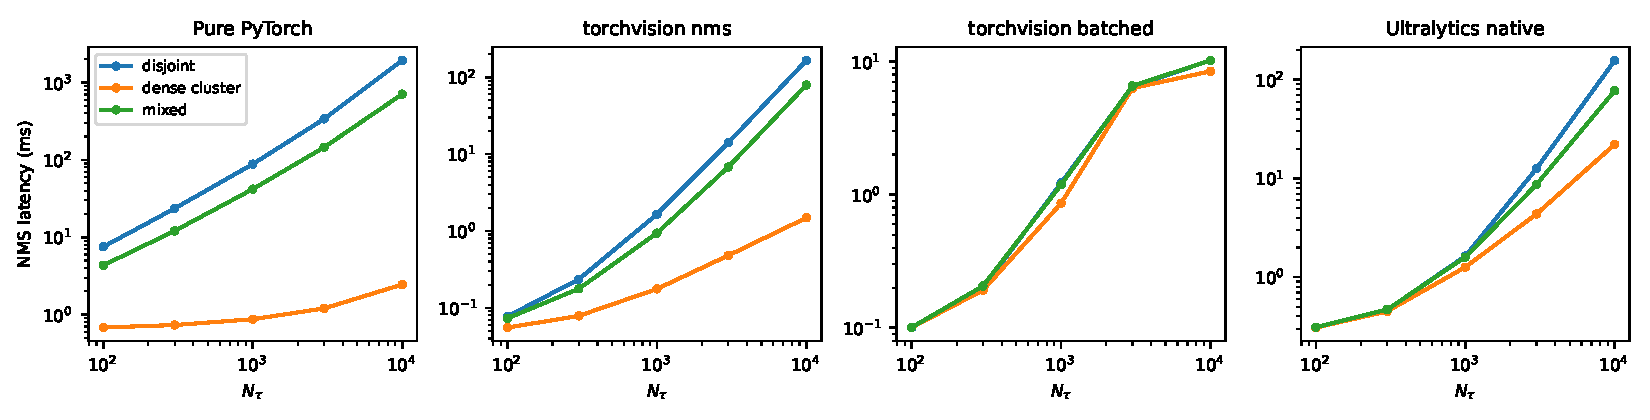
\includegraphics[width=\textwidth]{fig2_dose_response.pdf}
\caption{Độ trễ NMS theo $\Ntau$ trên profile laptop ghim lõi (lưới 10\,000 anchor, 80 lớp, không cap) cho bốn cài đặt và ba hình học hộp. Đường là trung vị; dải bóng là khoảng bootstrap 95\% qua các lần lặp. Cả hai trục là log.}
\label{fig:dose}
\end{figure*}
Trên head 2100 anchor, pure-PyTorch NMS với 2100 ứng viên rời mất 252~ms so với 0.894~ms với 10 ứng viên, tỷ số 281 (khoảng tin cậy 95\% từ 278 tới 285). Mỗi lần lặp toàn trình của pipeline pure-PyTorch với 2100 ứng viên tiêm (20/20; khoảng Wilson 95\% từ 0.84 tới 1.00) vượt mốc tham chiếu 100~ms. Bảng~\ref{tab:dose} cho tỷ số giữa $\Ntau=10^4$ và $\Ntau=10^2$ cho cả bốn cài đặt và ba hình học: ở cả 12 ô cận dưới của khoảng vượt $1+\mathrm{MDE}$, nhưng độ lớn trải từ 4.04 lần (pure PyTorch, cụm dày) tới 1356 lần (torchvision \texttt{nms}, rời), hơn hai bậc độ lớn giữa các cài đặt và hình học (Hình~\ref{fig:dose}).

\subsection{Q2: cài đặt, hình học và cap top-$k$}
\label{sec:q2}
% GENERATED by paper_en/tables_q3/make_tables_en.py -- DO NOT EDIT.
\begin{table*}[t]
\centering\small
\caption{Median NMS latency (ms) at $\Ntau=10^4$ (10\,000-anchor head, 80 classes) without a cap and with a top-300 cap, and the reduction factor (uncapped divided by capped; 95\% CI, bootstrap over repetitions).}
\label{tab:cap}
\begin{adjustbox}{max width=\textwidth}
\begin{tabular}{@{}llcccc@{}}
\toprule
Geometry & Implementation & No cap (ms) & Cap 300 (ms) & Reduction & 95\% CI \\
\midrule
Disjoint & pure PyTorch & 1929 & 23.4 & 82.5 & 82.2-82.7 \\
Disjoint & torchvision \texttt{nms} & 166 & 0.170 & 974 & 971-976 \\
Disjoint & torchvision batched & 10.2 & 0.194 & 52.5 & 52.4-52.6 \\
Disjoint & Ultralytics native & 157 & 0.457 & 342 & 337-346 \\
Mixed & pure PyTorch & 706 & 11.8 & 60.1 & 59.9-60.2 \\
Mixed & torchvision \texttt{nms} & 79.3 & 0.137 & 577 & 576-580 \\
Mixed & torchvision batched & 10.2 & 0.204 & 50.1 & 49.9-50.2 \\
Mixed & Ultralytics native & 77.7 & 0.471 & 165 & 164-168 \\
Dense cluster & pure PyTorch & 2.45 & 0.719 & 3.41 & 3.40-3.43 \\
Dense cluster & torchvision \texttt{nms} & 1.48 & 0.0752 & 19.7 & 19.6-19.8 \\
Dense cluster & torchvision batched & 8.45 & 0.193 & 43.7 & 43.6-43.8 \\
Dense cluster & Ultralytics native & 22.1 & 0.453 & 48.9 & 47.7-49.1 \\
\bottomrule
\end{tabular}
\end{adjustbox}
\end{table*}

\paragraph{Cài đặt và hình học ở cùng $\Ntau$ (H2).}
Ở $\Ntau=300$ trên head 2100 anchor với hình học hỗn hợp, pure-PyTorch NMS chậm hơn torchvision \texttt{nms} 80.3 lần (khoảng 76.4 tới 81.9), Ultralytics-native NMS chậm hơn 2.92 lần (2.79 tới 2.98), và torchvision \texttt{batched\_nms} chậm hơn 1.33 lần (1.24 tới 1.36). Ở $\Ntau=2100$, hộp rời tốn hơn cụm dày 192 lần cho vòng lặp pure-PyTorch (189 tới 196), 13.2 lần cho torchvision \texttt{nms} (12.9 tới 14.7), 1.78 lần cho Ultralytics (1.74 tới 1.82), và 1.01 lần cho torchvision \texttt{batched\_nms} (0.888 tới 1.07, chứa 1). Ở cùng $\Ntau$, chi phí NMS do đó có thể chênh nhau hơn hai bậc độ lớn.

\paragraph{Cap top-$k$ (H3).}
Bảng~\ref{tab:cap} cho trung vị độ trễ NMS ở $\Ntau=10^4$ khi không có cap và khi có cap 300 ứng viên. Cap giảm thời gian NMS ở cả 12 ô, nhưng hệ số giảm phụ thuộc mạnh vào cài đặt và hình học: từ 3.66 lần (pure PyTorch, cụm dày, nơi phần lớn hộp vốn đã bị ức chế sớm) tới 653 lần (torchvision \texttt{nms}, rời). Chọn 300 điểm cao nhất thuộc công đoạn lọc điểm, vốn mất 0.29~ms ở $\Ntau=10^4$ không cap và 0.46~ms khi có cap ở nhánh pure-PyTorch. Một pipeline cap số ứng viên trước NMS chặn phần lớn lợi ích mà một sự tăng $\Ntau$ có thể mang lại, bất kể bộ tối ưu.

\subsection{Q3: bao nhiêu ứng viên làm chậm toàn trình, và tấn công thật có đạt không}
\label{sec:q3}
% GENERATED by paper_en/tables_q3/make_tables_en.py -- DO NOT EDIT.
\begin{table*}[t]
\centering\small
\caption{Threshold $N^{*}$: the smallest grid level whose end-to-end ratio has a lower 95\% bound above $1+\mathrm{MDE}$ (full-pipeline injection, 20 images, no cap); ``$>$'': not reached. ``Measured'' uses the preregistered MDE (0.55\% at 320 px, 1.88\% at 640 px); ``MDE 0.69\%'' uses the repeated A/A. $^{\dagger}$Post hoc budget estimate. $^{\S}$Without flagged blocks (12/21 points flagged; 14 and 4 images remain).}
\label{tab:nstar}
\begin{adjustbox}{max width=\textwidth}
\begin{tabular}{@{}llccccccc@{}}
\toprule
 & & \multicolumn{3}{c}{320 px (grid 100, 300, 1000, 2100)} & \multicolumn{4}{c}{640 px (grid 300, 1000, 3000, 8400)} \\
\cmidrule(lr){3-5}\cmidrule(lr){6-9}
Implementation & Geometry & Measured & Predicted$^{\dagger}$ & Unflagged$^{\S}$ & Measured & MDE 0.69\% & Predicted$^{\dagger}$ & Unflagged$^{\S}$ \\
\midrule
pure PyTorch & disjoint & 100 & 100 & 100 & 300 & 300 & 300 & 300 \\
 & mixed & 100 & 100 & 100 & 300 & 300 & 300 & 300 \\
 & dense cluster & 300 & 100 & 300 & $>$8400 & $>$8400 & $>$8400 & $>$8400 \\
torchvision \texttt{nms} & disjoint & 1000 & 1000 & 2100 & 3000 & 3000 & 3000 & 3000 \\
 & mixed & 1000 & 1000 & 1000 & 8400 & 8400 & 3000 & 8400 \\
 & dense cluster & 1000 & 2100 & $>$2100 & $>$8400 & $>$8400 & $>$8400 & 8400 \\
torchvision batched & disjoint & 300 & 1000 & 300 & 1000 & 1000 & 3000 & 3000 \\
 & mixed & 1000 & 1000 & 1000 & 3000 & 1000 & 3000 & 3000 \\
 & dense cluster & 1000 & 1000 & 1000 & 3000 & 3000 & 3000 & 8400 \\
Ultralytics native & disjoint & 100 & 100 & 300 & 3000 & 3000 & 3000 & 3000 \\
 & mixed & 1000 & 100 & 1000 & 3000 & 3000 & 3000 & 3000 \\
 & dense cluster & 1000 & 100 & 1000 & 3000 & 3000 & 3000 & 3000 \\
\bottomrule
\end{tabular}
\end{adjustbox}
\end{table*}

\begin{figure*}[pos=!t]
\centering
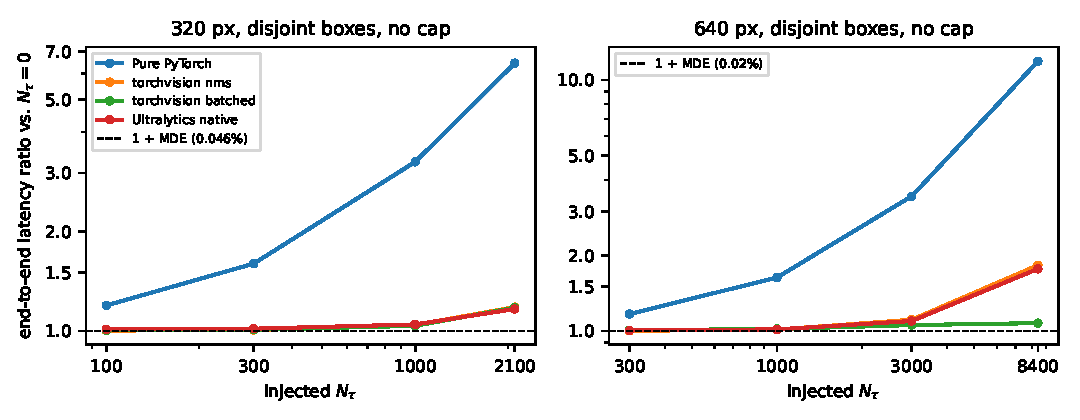
\includegraphics[width=\textwidth]{fig4_pipeline_nstar.pdf}
\caption{Tỷ số thời gian toàn trình so với $\Ntau=0$ khi tiêm ứng viên rời vào pipeline đầy đủ (20 ảnh, không cap top-$k$), ở 320 px và 640 px. Đường nét đứt là $1+\mathrm{MDE}$ toàn trình đăng ký trước; dải bóng là khoảng bootstrap 95\% qua ảnh. Cả hai trục là log.}
\label{fig:nstar}
\end{figure*}
\paragraph{Ngưỡng $N^{*}$ khi tiêm pipeline đầy đủ (H4).}
Chúng tôi tiêm các tập ứng viên tổng hợp vào pipeline đầy đủ (một forward pass thật trên ảnh, rồi lọc điểm và NMS) cho 20 ảnh held-out, bốn cài đặt, ba hình học, có và không cap top-300, ở 320 px ($\Ntau$ từ 0 tới 2100) và 640 px ($\Ntau$ từ 0 tới 8400). Ô $\Ntau=0$ của mỗi ảnh được đo ba lần và dùng làm mẫu số. $N^{*}$ là mức lưới nhỏ nhất mà tỷ số toàn trình có cận dưới 95\% (bootstrap qua ảnh) trên $1+\mathrm{MDE}$. Thiết kế, endpoint và quy tắc đọc được đăng ký trước. Ghim lõi qua kiểm chứng ở đầu và cuối phiên (0.97 và 0.83 lõi hiệu dụng); 12/21 điểm tham chiếu bị cờ vì trôi (lệch lớn nhất 30\%) và được giữ trong phân tích chính.

Với vòng lặp pure-PyTorch, thời gian toàn trình chậm đi phát hiện được từ 100 ứng viên ở 320 px và 300 ứng viên ở 640 px, và chậm 6.55 lần ở 2100 ứng viên (320 px) và 10.9 lần ở 8400 ứng viên (640 px), với hộp rời (Bảng~\ref{tab:nstar}, Hình~\ref{fig:nstar}). Với các kernel thư viện, ngưỡng cao hơn và mức tăng nhỏ hơn: torchvision \texttt{nms} cần 1000 ứng viên ở 320 px (1.11 lần toàn trình ở 2100) và 3000 ở 640 px (1.58 lần ở 8400). Ở 640 px, các ngưỡng tính với MDE đã đăng ký trước (1.88\%) và với MDE của A/A lặp lại (0.69\%) khác nhau ở 1 trong 12 ô không cap. Vì $N^{*}$ là mức đầu tiên vượt ngưỡng trên một lưới thưa, nên chỉ đọc nó như một bậc độ lớn; phân tích độ nhạy đã đăng ký trước, bỏ các khối bị cờ, đẩy nó lên một mức lưới ở một số ô. Sàn nhiễu trong phiên của phép tiêm (bản sao thứ hai của ô $\Ntau=0$ so với bản đầu) là 2.5--3.2\% ở 320 px và 3.3--6.3\% ở 640 px, cao hơn MDE của các A/A riêng vì mỗi ô chỉ có 3--5 lần lặp; với sàn nhiễu này các ngưỡng sẽ cao hơn. Cap top-300 chặn phần lớn mức tăng cho các kernel thư viện; vòng lặp pure-PyTorch vẫn chậm 1.64 lần (320 px) và 1.20 lần (640 px) ở $\Ntau$ lớn nhất với hộp rời, vì 300 hộp vẫn là nhiều cho một vòng lặp Python.

\paragraph{Ngưỡng tính bằng mili-giây.}
\label{sec:threshold}
Từ $R \approx 1 + \Delta t_{\mathrm{NMS}}/t_{\mathrm{total}}$ (Mục~\ref{sec:amdahl}), riêng mức tăng ở NMS đưa tỷ số ước lượng vượt $1+\mathrm{MDE}$ khi
\begin{equation}
\Delta t_{\mathrm{NMS}} > \Delta t^{*} = \mathrm{MDE} \times t_{\mathrm{total}} ,
\end{equation}
trong đó $\mathrm{MDE}$ và $t_{\mathrm{total}}$ phải dùng chung định nghĩa toàn trình của phép so sánh. Với phiên đo patch ($t_{\mathrm{total}}$ sạch là 50.8~ms ở 320 px và 166~ms ở 640 px với torchvision; MDE lấy từ A/A, vì phiên này không có hai nhánh sạch), $\Delta t^{*}$ là 0.28~ms ở 320 px và 1.1~ms ở 640 px. Baseline gradient là điều kiện duy nhất rõ ràng làm tăng $\Ntau$. Với torchvision \texttt{nms} nó thêm 0.017~ms vào công đoạn NMS (micro-benchmark), dưới $\Delta t^{*}$, nên mô hình ngân sách \emph{dự đoán} một tỷ số toàn trình chỉ 1.0003, dưới $1+\mathrm{MDE}$. Với vòng lặp pure-PyTorch nó thêm 0.99~ms, trên $\Delta t^{*}$ (0.29~ms), và mô hình \emph{dự đoán} 1.0199, trên $1+\mathrm{MDE}$. Đây là dự đoán của mô hình ngân sách, không phải đo toàn trình (Mục~\ref{sec:attackdesign}).

% GENERATED by paper_en/tables_q3/make_tables_en.py -- DO NOT EDIT.
\begin{table*}[t]
\centering\small
\caption{Effect of the frozen patches relative to clean images of the same canvas, 100 images $\times$ 5 seeds, one drift-gated session (10/10 blocks accepted at the first attempt). All ratios are measured: mean over image $\times$ seed pairs, 95\% CI from a two-level bootstrap. NMS: torchvision, $\tau=0.01$. ``(above)'': lower bound $>1+\mathrm{MDE}$; MDE in-session (two clean arms), torchvision / pure PyTorch.}
\label{tab:patches}
\begin{adjustbox}{max width=\textwidth}
\begin{tabular}{@{}lcccccc@{}}
\toprule
Condition & $\Ntau$ ratio ($\tau$=0.01) & $\Ntau$ ratio ($\tau$=0.25) & NMS ratio & End-to-end, \texttt{nms} & End-to-end, pure PyTorch & MDE (\%) \\
\midrule
320 px, 64-px patch, $\tau_{\mathrm{obj}}$ 0.01 & 1.04 (0.99-1.10) & 0.94 (0.86-1.03) & 0.997 (0.985-1.009) & 1.0010 (1.0001-1.0019) & 1.0001 (0.9985-1.0017) & 0.20 / 0.20 \\
320 px, 64-px patch, $\tau_{\mathrm{obj}}$ 0.25 & 1.04 (0.99-1.09) & 0.95 (0.86-1.05) & 0.997 (0.984-1.008) & 1.0008 (0.9999-1.0017) & 0.9998 (0.9981-1.0014) & 0.20 / 0.20 \\
Random search (320 px) & 1.03 (0.98-1.08) & 0.95 (0.86-1.07) & 0.997 (0.984-1.009) & 1.0008 (0.9998-1.0017) & 1.0000 (0.9983-1.0016) & 0.20 / 0.20 \\
GA, centre placement (320 px) & 1.05 (0.99-1.10) & 0.90 (0.83-0.99) & 1.007 (0.995-1.019) & 1.0007 (0.9998-1.0017) & 1.0005 (0.9989-1.0021) & 0.20 / 0.20 \\
GA, random placement (320 px) & 1.06 (1.03-1.10) & 0.93 (0.87-0.97) & 1.005 (0.995-1.014) & 1.0009 (1.0000-1.0018) & 1.0011 (0.9997-1.0024) & 0.20 / 0.20 \\
Gradient ascent (320 px) & 2.39 (2.09-2.74) & 6.81 (4.72-9.44) & 1.247 (1.210-1.285) & 1.0018 (1.0009-1.0028) & 1.0203 (1.0177-1.0229) (above) & 0.20 / 0.20 \\
640 px, 128-px patch, $\tau_{\mathrm{obj}}$ 0.01 & 1.07 (1.00-1.16) & 0.94 (0.89-0.99) & 0.996 (0.976-1.013) & 0.9979 (0.9915-1.0041) & 0.9972 (0.9909-1.0035) & 1.14 / 1.10 \\
640 px, 64-px patch, $\tau_{\mathrm{obj}}$ 0.01 & 1.05 (1.02-1.08) & 0.96 (0.92-1.00) & 1.010 (1.001-1.018) & 1.0010 (0.9941-1.0080) & 1.0007 (0.9938-1.0075) & 1.14 / 1.10 \\
\bottomrule
\end{tabular}
\end{adjustbox}
\end{table*}

\begin{figure*}[pos=!t]
\centering
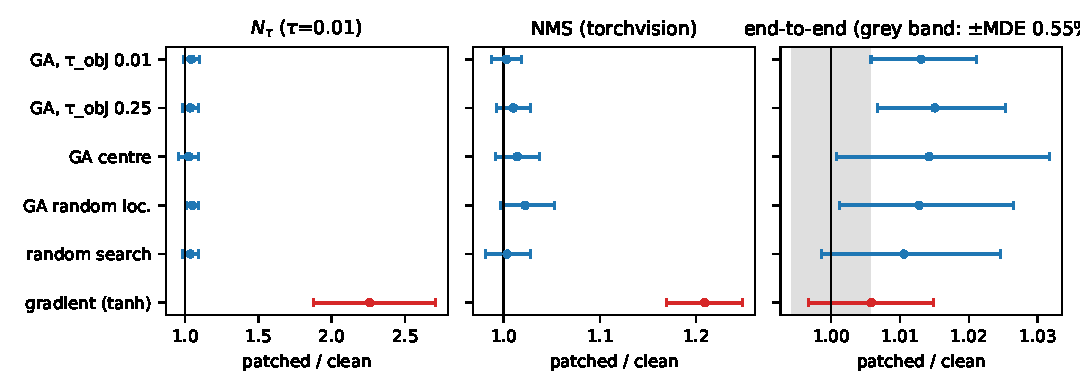
\includegraphics[width=\textwidth]{fig6_patch_effects.pdf}
\caption{Tỷ số giữa ảnh dán patch và ảnh sạch ở 320 px. Trái và giữa: $\Ntau$ và công đoạn NMS (torchvision), đo được, khoảng bootstrap hai tầng 95\%. Phải: tỷ số toàn trình \emph{dự đoán} bởi mô hình ngân sách $1+\Delta t_{\mathrm{NMS}}/t_{\mathrm{total}}$ (vòng tròn: torchvision \texttt{nms}; vuông: pure PyTorch), không đo; dải xám là $\pm$ MDE A/A toàn trình.}
\label{fig:patches}
\end{figure*}
\paragraph{Patch thật.}
Mỗi điều kiện dùng 100 ảnh held-out và năm seed patch. Các tỷ số $\Ntau$ và tỷ số công đoạn NMS trong Bảng~\ref{tab:patches} là phép đo; cột toàn trình là một \emph{dự đoán} của mô hình ngân sách (Bảng~\ref{tab:dev}). Các patch từ giải thuật di truyền không làm tăng $\Ntau$ đáng kể (Hình~\ref{fig:patches}): trung vị $\Ntau$ ở $\tau=0.01$ đi từ 86.5 (sạch) xuống 85.5 và 85.0 ở 320 px, các khoảng của tỷ số chứa 1, và random search cùng hai baseline đặt vị trí cho cùng bức tranh. Các giá trị này dưới mọi ngưỡng $N^{*}$ đo trên pipeline YOLOv8n ở 320 px (thấp nhất là 100, Bảng~\ref{tab:nstar}); so sánh chỉ là một bậc độ lớn, vì $N^{*}$ đo bằng ứng viên tổng hợp hình học kiểm soát. Ở 640 px trung vị $\Ntau$ tăng từ 119.0 lên 134.0 (patch 128 px) và 138.5 (patch 64 px), cũng dưới $N^{*}$ thấp nhất ở 640 px (300). Mô hình ngân sách \emph{dự đoán} không patch GA nào làm tăng thời gian toàn trình trên $1+\mathrm{MDE}$ với bất kỳ cài đặt nào. Baseline gradient nâng trung vị $\Ntau$ từ 86.5 lên 165.0 và công đoạn NMS torchvision lên 1.228 lần, nhưng tỷ số toàn trình \emph{dự đoán} của nó chỉ vượt $1+\mathrm{MDE}$ với vòng lặp pure-PyTorch. Một lần đếm lại post hoc từ dữ liệu lịch sử đã lưu, chỉ đếm ứng viên và không đo thời gian, cho cùng bức tranh trên năm bộ phát hiện YOLO (YOLOv8n, YOLOv8s, YOLO11n, YOLO11s, YOLOv12n) khi chèn năm patch SG-GA của một lượt chạy trước: tỷ số $\Ntau$ là 1.022 tới 1.036 với các khoảng chứa 1, và trung vị $\Ntau$ có patch (85.0 tới 104.0) vẫn ở mức của ảnh sạch.

% GENERATED by paper_en/tables_q3/make_tables_en.py -- DO NOT EDIT.
\begin{table*}[t]
\centering\small
\caption{Adaptive variants of two whole-image attacks (YOLOv5s, 640 px, 50 images $\times$ 5 seeds, frequency-locked core). Median $\Ntau$ clean $\to$ perturbed and mean of the per-image $\Ntau$ ratios ($\tau=0.25$); end-to-end ratio (95\% CI, two-level bootstrap); ``above MDE'': lower bound $>1+\mathrm{MDE}$ of the session. $^{\dagger}$Post hoc: threshold $\Delta t^{*}$ and median NMS increase.}
\label{tab:attacks}
\begin{adjustbox}{max width=\textwidth}
\begin{tabular}{@{}lcclccccc@{}}
\toprule
Variant & $\Ntau$ clean $\to$ attack & $\Ntau$ ratio (95\% CI) & Implementation & End-to-end ratio (95\% CI) & MDE (\%) & Above MDE & $\Delta t^{*}$ (ms)$^{\dagger}$ & $\Delta t_{\mathrm{NMS}}$ (ms)$^{\dagger}$ \\
\midrule
Overload & 45.0 $\to$ 5578.5 & 389 (135-753) & torchvision \texttt{nms} & 1.018 (1.000-1.038) & 2.82 & no & 7.7 & 8.6 \\
 & &  & torchvision batched & 1.013 (0.993-1.033) & 2.82 & no & 7.7 & 5.9 \\
 & &  & Ultralytics native & 1.020 (1.001-1.040) & 2.80 & no & 7.7 & 8.4 \\
Phantom Sponges & 45.0 $\to$ 4811.5 & 340 (104-678) & torchvision \texttt{nms} & 1.016 (0.997-1.036) & 2.82 & no & 7.7 & 9.6 \\
 & &  & torchvision batched & 1.017 (0.998-1.036) & 2.82 & no & 7.7 & 9.5 \\
 & &  & Ultralytics native & 1.020 (1.001-1.040) & 2.80 & no & 7.7 & 10 \\
\bottomrule
\end{tabular}
\end{adjustbox}
\end{table*}

% GENERATED by paper_en/tables_q3/make_tables_en.py -- DO NOT EDIT.
\begin{table*}[t]
\centering\small
\caption{\textbf{Post hoc}, YOLOv5s (640 px): decomposition of the latency increase of the whole-image attack variants per image $\times$ seed pair (ms; 95\% CI, two-level bootstrap). The remainder is $\Delta t_{\mathrm{total}}-\Delta t_{\mathrm{NMS}}$; the raw records do not separate its stages.}
\label{tab:decomp}
\begin{adjustbox}{max width=\textwidth}
\begin{tabular}{@{}llcccc@{}}
\toprule
Variant & Implementation & $\Delta t_{\mathrm{total}}$ & $\Delta t_{\mathrm{NMS}}$ & Remainder & Remainder / $\Delta t_{\mathrm{total}}$ (\%) \\
\midrule
Overload & torchvision \texttt{nms} & 10.5 (6.8-14) & 5.24 (4.1-6.4) & 5.26 (1.8-8.7) & 50 \\
Overload & torchvision batched & 9.06 (5.3-13) & 4.91 (3.4-6.5) & 4.15 (0.82-7.6) & 46 \\
Overload & Ultralytics native & 10.7 (6.6-15) & 7.04 (5.7-8.4) & 3.66 ($-$0.18-7.6) & 34 \\
Phantom Sponges & torchvision \texttt{nms} & 10.0 (6.5-13) & 5.44 (4.3-6.6) & 4.58 (1.4-7.7) & 46 \\
Phantom Sponges & torchvision batched & 9.77 (6.0-14) & 5.99 (4.8-7.2) & 3.77 (0.31-7.9) & 39 \\
Phantom Sponges & Ultralytics native & 10.2 (6.0-14) & 6.86 (5.5-8.2) & 3.29 ($-$0.50-7.2) & 32 \\
\bottomrule
\end{tabular}
\end{adjustbox}
\end{table*}

\begin{figure*}[pos=!t]
\centering
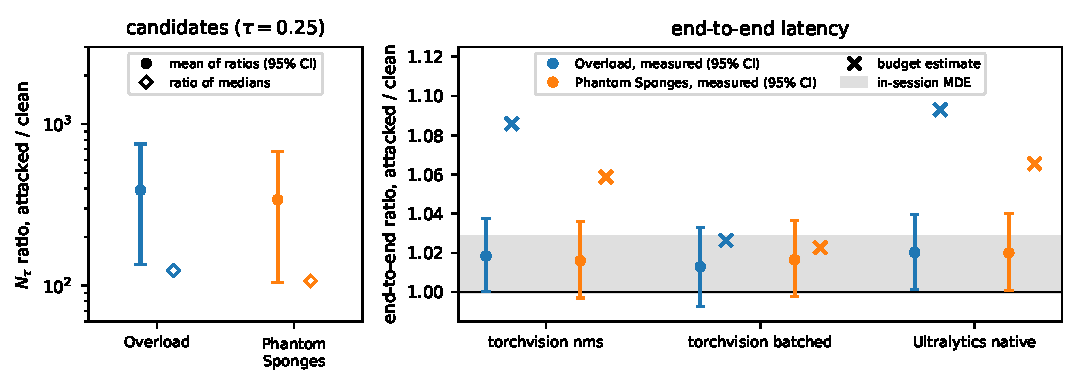
\includegraphics[width=\textwidth]{fig9_attacks.pdf}
\caption{Các biến thể thích ứng của hai tấn công toàn ảnh (YOLOv5s, 640 px) dưới giao thức ghim lõi. Trái: tỷ số $\Ntau$ ($\tau=0.25$) so với ảnh sạch, thang log. Phải: tỷ số toàn trình đo được (chấm, khoảng 95\%) và dự đoán của mô hình Amdahl đăng ký trước (dấu chéo) theo cài đặt NMS; dải xám là MDE trong phiên.}
\label{fig:attacks}
\end{figure*}
\paragraph{Các biến thể tấn công toàn ảnh.}
\label{sec:attacks}
Phiên qua kiểm chứng ghim ở đầu và cuối (0.85 và 0.98) và 0/11 điểm tham chiếu bị cờ (lệch tối đa 2.0\%). Các nhiễu nâng $\Ntau$ ở $\tau=0.25$ lên 340 tới 389 lần (Bảng~\ref{tab:attacks}, Hình~\ref{fig:attacks}); ở $\tau=0.01$ trung vị $\Ntau$ tăng từ 253.5 lên 11674.0 (biến thể Overload) và 14487.5 (biến thể Phantom Sponges). Công đoạn NMS của các kernel thư viện tăng từ trung vị 0.048--0.35~ms lên 4.5--7.8~ms, và của vòng lặp pure-PyTorch từ 0.51~ms lên 55--79~ms. Dù vậy, thời gian toàn trình với các kernel thư viện chỉ tăng từ trung vị 315--317~ms lên 324--328~ms: tỷ số 1.029 tới 1.034, với khoảng loại trừ 1. Sàn nhiễu trong phiên là 1.97--2.44\%, nên mức tăng vượt sàn nhiễu với torchvision \texttt{nms} nhưng không với hai kernel kia. Mọi so sánh ở đây dùng ngưỡng của chính YOLOv5s, không phải ngưỡng $N^{*}$ của YOLOv8n: với $t_{\mathrm{total}}$ và MDE của phiên YOLOv5s, $\Delta t^{*}$ là 6.2--7.7~ms, trong khi mức tăng trung vị của công đoạn NMS là 4.3--7.4~ms, dưới $\Delta t^{*}$ ở mọi ô (post hoc). Một phân rã theo từng cặp ảnh $\times$ seed (Bảng~\ref{tab:decomp}, post hoc, không đo mới) cho thấy NMS chỉ giải thích một phần mức tăng toàn trình: phần còn lại là 3.3--5.3~ms, 32--50\% mức tăng, với khoảng loại trừ 0 ở 4/6 ô. Phần còn lại nằm ở forward pass, giải mã, lọc điểm và dựng đầu vào NMS; các bản ghi thô không tách riêng các công đoạn này. Kết luận này chỉ áp dụng cho các biến thể này, YOLOv5s và một lõi CPU: ở cấu hình đó NMS vẫn chỉ chiếm 1.4--2.3\% thời gian toàn trình sau mức tăng. Áp biểu thức Amdahl cho vòng lặp pure-PyTorch (thời gian toàn trình không đo vì chi phí) cho một mức tăng toàn trình suy ra khoảng 17--25\%; đây là suy luận từ mô hình, không phải đo.

\subsection{Q4: một bộ dự đoán chỉ từ $\Ntau$ chính xác đến đâu}
\label{sec:q4}
\begin{figure*}[pos=!t]
\centering
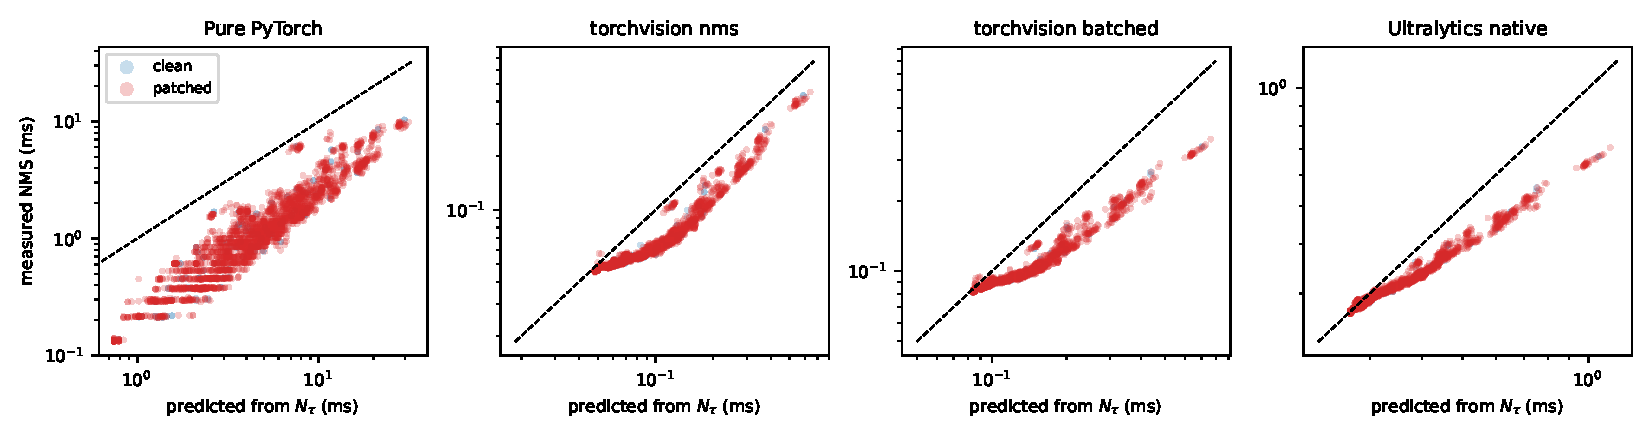
\includegraphics[width=\textwidth]{fig3_pred_vs_measured.pdf}
\caption{Độ trễ NMS đo được của các tập ứng viên thật ($\tau=0.01$, điều kiện 320 px) so với dự đoán chỉ từ $\Ntau$ dùng đường cong dose-response hình học hỗn hợp, theo cài đặt. Đường nét đứt là đẳng thức. Chấm xanh là ảnh sạch, chấm đỏ là ảnh dán patch.}
\label{fig:pred}
\end{figure*}
\paragraph{Thời gian NMS của các tập ứng viên thật.}
Với mỗi đơn vị đo của lượt patch 320 px có $\Ntau>0$, chúng tôi dự đoán $t_{\mathrm{NMS}}$ chỉ từ $\Ntau$ bằng cách nội suy, trên thang log--log, đường liều--đáp ứng của cài đặt tương ứng (đầu 2100 anchor, hình học hỗn hợp), và báo cáo trung vị và phân vị 90 của $|\ln(t_{\mathrm{meas}}/t_{\mathrm{pred}})|$ (Hình~\ref{fig:pred}). Các đại lượng này dùng công đoạn NMS được đo thời gian riêng, không bị bước chèn ảnh hưởng, và không có ngưỡng đạt/không đạt nào được đặt trước. Qua 3347 điểm đo, sai số trung vị và bách phân vị 90 là 0.05 và 0.15 cho Ultralytics native, 0.15 và 0.40 cho torchvision batched, 0.33 và 0.47 cho torchvision \texttt{nms}, và 1.38 và 1.73 cho pure PyTorch (sai số điển hình khoảng bốn lần cho cái sau). Tỷ lệ điểm đo nằm giữa đường hộp rời và đường cụm dày là 0.44 với Ultralytics native, 0.35 với torchvision batched, 0.93 với torchvision \texttt{nms} và 0.76 với pure PyTorch. Giữa các ảnh sạch, tương quan hạng của $\Ntau$ với thời gian NMS cao (0.84 tới 0.94 tùy cài đặt), còn với thay đổi trong cùng một ảnh do patch gây ra thì thấp hơn (0.27 tới 0.73 trên các điều kiện 320 px): $\Ntau$ xếp hạng chi phí giữa các ảnh tốt hơn là xếp hạng tác động của một chỉnh sửa trên một ảnh. Cả hai tương quan đều mô tả. Trên các biến thể tấn công toàn ảnh, nội suy chỉ từ $\Ntau$ sai 0.47 tới 1.78 (sai số log trung vị), vì các ứng viên do tấn công tạo ra chồng lấn mạnh và bị ức chế nhanh hơn hình học hỗn hợp tổng hợp.

% GENERATED by paper_en/tables_q3/make_tables_en.py -- DO NOT EDIT.
\begin{table*}[t]
\centering\small
\caption{Median error $|\ln(t_{\mathrm{meas}}/t_{\mathrm{pred}})|$ of $M_N$ and $M_{NK}$, fitted on the injection cells, on the real candidate sets of all arms of the patch session ($\tau=0.01$), and the difference $\Delta$ ($M_N$ minus $M_{NK}$) with a 95\% two-level bootstrap CI (images, units within images). $\Delta>0$ means that adding $K$ reduces the error.}
\label{tab:nk}
\begin{adjustbox}{max width=\textwidth}
\begin{tabular}{@{}lccc@{}}
\toprule
Implementation & $M_N$ & $M_{NK}$ & $\Delta$ (95\% CI) \\
\midrule
\multicolumn{4}{@{}l}{\textit{Real candidate sets of the patch session, \textbf{post hoc} (4397 units, 100 images)}} \\
pure PyTorch & 1.00 & 0.33 & 0.67 (0.55 to 0.74) \\
torchvision \texttt{nms} & 0.65 & 0.63 & 0.02 ($-$0.08 to 0.12) \\
torchvision batched & 0.70 & 2.07 & $-$1.37 ($-$1.47 to $-$1.26) \\
Ultralytics native & 0.46 & 2.48 & $-$2.02 ($-$2.12 to $-$1.91) \\
\bottomrule
\end{tabular}
\end{adjustbox}
\end{table*}

\paragraph{Hình học có giải thích phần sai còn lại không?}
\label{sec:nk}
Chúng tôi so hai mô hình log-tuyến tính khớp theo từng cài đặt trên các ô của phép tiêm tổng hợp: $M_N$, $\ln t_{\mathrm{NMS}} = a + b\ln\Ntau$, và $M_{NK}$, thêm một số hạng $c\ln\max(K,1)$ với $K$ là số hộp NMS giữ lại. $K$ là một proxy cho hình học nhưng chỉ biết sau khi NMS đã chạy, nên $M_{NK}$ là một phân rã chứ không phải một bộ dự đoán triển khai được. Đặc tả được cố định trước khi khớp; đánh giá xác nhận dùng các tập ứng viên thật ở 640 px, còn đánh giá ở 320 px là post hoc (Bảng~\ref{tab:nk}). Với vòng lặp pure-PyTorch, thêm $K$ giảm sai số khoảng một nửa, đúng như mô hình chi phí dự đoán; với torchvision \texttt{nms} không phát hiện cải thiện; với hai cài đặt class-aware $M_{NK}$ rõ ràng tệ hơn, vì một mô hình học từ tập tổng hợp (80 lớp ngẫu nhiên) ngoại suy kém sang phân bố lớp của ứng viên thật. Trên các biến thể tấn công toàn ảnh, $M_N$ sai 0.30 tới 0.43 và thêm $K$ chỉ giúp torchvision \texttt{nms} (chênh 0.15; 0.05 tới 0.24). $\Ntau$ một mình không đủ để dự đoán thời gian NMS, và một mô hình hiệu chuẩn hoàn toàn trên ứng viên tổng hợp không thay thế được phép đo trên ứng viên thật.

% GENERATED by paper_en/tables_q3/make_tables_en.py -- DO NOT EDIT.
\begin{table*}[t]
\centering\small
\caption{Budget estimate $R_{\mathrm{pred}} = 1+\Delta t_{\mathrm{NMS}}/t_{\mathrm{total}}$ against the measured ratio $R_{\mathrm{meas}}$; error is $|\ln(R_{\mathrm{meas}}/R_{\mathrm{pred}})|$. Part A (post hoc): full-pipeline injection, 156 cells, median error 0.012, 90th percentile 0.040; predicted and measured $N^{*}$ agree in 35/48 cells. Part B: whole-image attack variants on YOLOv5s, preregistered rule (upper 95\% bound of the median error $<0.05$); 3/6 cells pass.}
\label{tab:amdahl}
\begin{adjustbox}{max width=\textwidth}
\begin{tabular}{@{}lccccc@{}}
\toprule
 & $R_{\mathrm{pred}}$ & $R_{\mathrm{meas}}$ & Error (95\% CI) & $N^{*}$ predicted / measured & Rule \\
\midrule
\multicolumn{6}{@{}l}{\textit{A. Full-pipeline injection, \textbf{post hoc}; 320 px, disjoint boxes, no cap, $\Ntau=2100$}} \\
pure PyTorch & 6.44 & 6.57 & 0.020 & 100 / 100 & - \\
torchvision \texttt{nms} & 1.10 & 1.11 & 0.009 & 1000 / 1000 & - \\
torchvision batched & 1.14 & 1.20 & 0.056 & 1000 / 300 & - \\
Ultralytics native & 1.12 & 1.14 & 0.018 & 100 / 300 & - \\
\multicolumn{6}{@{}l}{\textit{A. Full-pipeline injection, \textbf{post hoc}; 640 px, disjoint boxes, no cap, $\Ntau=8400$}} \\
pure PyTorch & 10.5 & 10.9 & 0.035 & 300 / 300 & - \\
torchvision \texttt{nms} & 1.54 & 1.57 & 0.020 & 3000 / 3000 & - \\
torchvision batched & 1.06 & 1.09 & 0.023 & 3000 / 1000 & - \\
Ultralytics native & 1.56 & 1.58 & 0.015 & 3000 / 3000 & - \\
\midrule
\multicolumn{6}{@{}l}{\textit{B. Whole-image attack variants (YOLOv5s, 640 px), preregistered model and rule}} \\
Overload, torchvision \texttt{nms} & 1.067 & 1.034 & 0.046 (0.034-0.058) & - & \textbf{fail} \\
Overload, torchvision batched & 1.027 & 1.029 & 0.022 (0.017-0.028) & - & pass \\
Overload, Ultralytics native & 1.098 & 1.034 & 0.067 (0.049-0.088) & - & \textbf{fail} \\
Phantom Sponges, torchvision \texttt{nms} & 1.042 & 1.032 & 0.031 (0.024-0.038) & - & pass \\
Phantom Sponges, torchvision batched & 1.023 & 1.031 & 0.024 (0.019-0.030) & - & pass \\
Phantom Sponges, Ultralytics native & 1.065 & 1.033 & 0.044 (0.033-0.054) & - & \textbf{fail} \\
\bottomrule
\end{tabular}
\end{adjustbox}
\end{table*}

\paragraph{Mô hình Amdahl cho thời gian toàn trình.}
Trên phép tiêm toàn pipeline, mô hình Amdahl với các đường cong tiêm (đầu 2100 và 8400 anchor) và thời gian toàn trình sạch của cùng phiên dự đoán tỷ số đo được với sai số log trung vị 0.012 trên 156 ô, và ngưỡng dự đoán bằng ngưỡng đo được ở 35 trong 48 ô (Bảng~\ref{tab:amdahl}; ngưỡng đo được tính theo cách gộp của mô hình, một phân tích độ nhạy; kết quả ngưỡng chính là Bảng~\ref{tab:nstar}). Phân tích này là post hoc: mô hình được viết sau khi thấy phép tiêm. Trên các biến thể tấn công toàn ảnh, với đặc tả và quy tắc cố định trước khi đo, mô hình đạt quy tắc ở 3/6 ô (torchvision batched với cả hai biến thể, và torchvision \texttt{nms} với biến thể Phantom Sponges) và trượt ở 3 ô (torchvision \texttt{nms} với biến thể Overload, và Ultralytics native với cả hai biến thể, nơi nó dự đoán tỷ số lớn hơn đo được). Có hai lý do khả dĩ, cả hai từ phân tích post hoc. Thứ nhất, đường cong hình học hỗn hợp tổng hợp ước lượng quá cao chi phí NMS của ứng viên thật (sai số nội suy ở trên). Thứ hai, ngay cả khi thay đường cong bằng thời gian NMS đo được của chính tập ứng viên, mô hình chỉ-NMS vẫn hụt (sai số log 0.023--0.026), vì các công đoạn khác cũng tăng theo $\Ntau$ (lọc điểm trên 25\,200 hàng và dựng đầu vào NMS). Kết quả 3/6 do đó không đủ để coi mô hình đúng trên tấn công thật; nó cho thấy mô hình cần các công đoạn này và một đường cong có hình học gần ứng viên thật hơn.

\subsection{Kiểm chéo trên một board Arm nơi hậu xử lý chiếm ưu thế}
\label{sec:pi3b}
\begin{table*}[pos=!t]
\centering\small
\caption{Tỷ số độ trễ toàn trình trên Raspberry Pi 3B ở xung nhịp 600~MHz đã khai báo (YOLOv8n-seg, 20 cặp ảnh đóng băng; trung bình nhân của tỷ số theo ảnh, CI 95\% từ 20\,000 lần lấy mẫu lại ảnh). Hai phiên là hai điều kiện đăng ký trước riêng và không được gộp.}
\label{tab:pi3b}
\begin{adjustbox}{max width=\textwidth}
\begin{tabular}{@{}lcc@{}}
\toprule
Phiên & Bị tấn công / sạch & Có cap / bị tấn công \\
\midrule
Bốn luồng, không thiết bị USB & 1.798 [1.747, 1.848] & 0.729 [0.713, 0.746] \\
Một luồng, gắn SSD USB nằm im & 1.967 [1.902, 2.030] & 0.699 [0.682, 0.718] \\
\bottomrule
\end{tabular}
\end{adjustbox}
\end{table*}
\begin{figure*}[pos=!t]
\centering
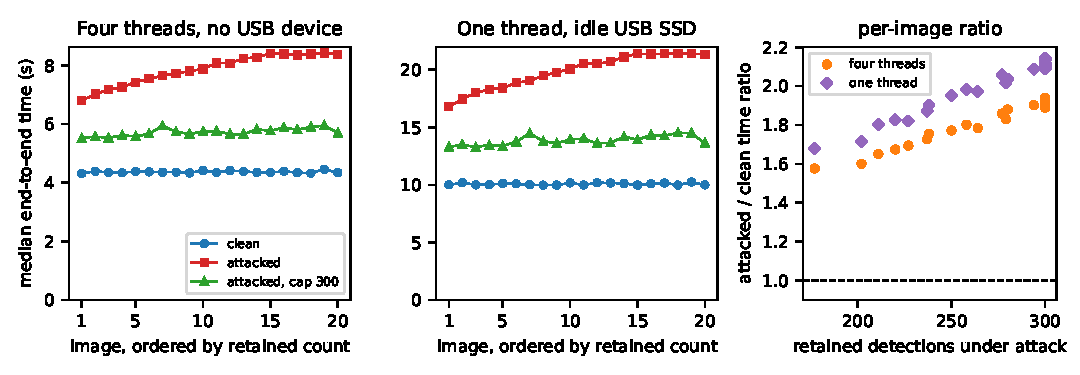
\includegraphics[width=\textwidth]{fig10_pi3b.pdf}
\caption{Raspberry Pi 3B ở xung nhịp 600~MHz đã khai báo (YOLOv8n-seg, 20 cặp ảnh đóng băng). Trái và giữa: trung vị thời gian toàn trình theo ảnh cho đầu vào sạch, bị tấn công và bị tấn công có cap (300 ứng viên) ở hai phiên đạt cổng; ảnh xếp theo số phát hiện được giữ lại khi bị tấn công. Phải: tỷ số bị tấn công/sạch theo ảnh so với số phát hiện được giữ lại khi bị tấn công. Mang tính mô tả; hai phiên không được gộp và hình không tách NMS khỏi việc dựng mask.}
\label{fig:pi3b}
\end{figure*}
Các kết quả phát hiện ở trên đến từ một cấu hình trong đó forward pass chiếm ưu thế. Để quan sát chế độ ngược lại trên một thiết bị Arm, chúng tôi chạy lại, theo các giao thức đăng ký trước riêng, 20 nhiễu toàn ảnh đã đóng băng (PGD, $L_\infty=16/255$, 100 bước, cỡ bước $2/255$) trên YOLOv8n-seg, một mô hình phân đoạn thực thể có hậu xử lý dựng một mask độ phân giải đầy đủ cho mỗi phát hiện được giữ lại, nên khối lượng hậu xử lý phụ thuộc số phát hiện được giữ lại cũng như $\Ntau$. Thiết bị là một Raspberry Pi 3B (bốn lõi Cortex-A53) bị firmware ép xung nhịp về 600~MHz do thiếu áp; đây là điểm vận hành đã khai báo, xung nhịp lấy mẫu là 600~MHz suốt phiên, và không quy đổi sang xung nhịp nào khác. Suy luận là FP32 ở $640\times640$ với ngưỡng tin cậy 0.25, IoU 0.45 và backend NMS torchvision cố định, và endpoint là thời gian từ tensor đã chuẩn bị tới khi trả về mask gốc. Trên mô hình này các nhiễu nâng trung vị số phát hiện được giữ lại từ 2.5 lên 270, và các số đếm trên board khớp với trên laptop ở cả 20 cặp.

Bảng~\ref{tab:pi3b} cho hai phiên đạt mọi cổng chất lượng đã đăng ký trước (kiểm tải, trôi tham chiếu, tắt swap, sàn nhiễu A/A, khôi phục cấu hình). Với bốn luồng ghim vào bốn lõi (720 lần đo, không điểm nào trong 22 điểm tham chiếu bị cờ, tỷ số A/A 0.9990), đầu vào bị tấn công mất thời gian gấp 1.798 lần đầu vào sạch (CI 95\% từ 1.747 tới 1.848; kiểm định đảo dấu chính xác $p=0.00000191$). Với một lõi được ghim, tỷ số là 1.967 (1.902 tới 2.030; cả 20 ảnh đều dương), và trung vị thời gian toàn trình là 10.05~s khi sạch so với 20.30~s khi bị tấn công. Phiên một lõi là một điều kiện khai báo riêng: có gắn một SSD USB nằm im, cấp nguồn riêng và không mount, bộ đếm sector ghi của nó giữ nguyên bằng không suốt phiên, và kết quả của nó không được gộp với phiên bốn luồng. Ở phiên bốn luồng, trung vị tỷ trọng forward pass theo ảnh giảm từ 98.6\% trên đầu vào sạch xuống 54.0\% trên đầu vào bị nhiễu: sau tấn công gần một nửa thời gian là hậu xử lý, đúng chế độ mà H4 cho phép một tác động toàn trình nhìn thấy được. Giới hạn số ứng viên đưa vào NMS ở 300 giảm thời gian toàn trình khi bị tấn công xuống còn 0.729 (0.713 tới 0.746) và 0.699 (0.682 tới 0.718) so với khi không cap, cùng chiều với H3. Hình~\ref{fig:pi3b} cho thời gian theo từng ảnh: thời gian sạch gần như không đổi giữa các ảnh, còn thời gian khi bị tấn công tăng theo số phát hiện được giữ lại (177 tới 300 mỗi ảnh), cho tỷ số theo ảnh từ 1.577 tới 1.939 với bốn luồng và từ 1.678 tới 2.144 với một luồng. Xu hướng giữa các ảnh này chỉ mang tính mô tả.

Kết quả này có giới hạn rõ ràng. Phiên thành phần lẽ ra tách NMS khỏi việc dựng mask đã hoàn tất 705 lần đo nhưng không đạt các cổng độ chính xác NMS (tỷ số A/A 0.9476, log-MDE 0.1652), trong khi đối chứng mask của nó đạt (0.9941, log-MDE 0.0271); vì vậy cổng chung không đạt, và chúng tôi không quy mức chậm cho NMS, cho việc dựng mask hay cho bất kỳ tỷ lệ chia nào giữa hai phần. Hai giao thức trước đó trên cùng board không đạt cổng swap hoặc cổng độ chính xác pilot và được giữ lại như các lượt bị loại. 20 cặp là đầu vào đóng băng dùng lại giữa các phiên, không phải một cohort độc lập; các khoảng tin cậy chỉ lấy mẫu lại ảnh và không phủ seed nhiễu, board hay điều kiện nguồn. Các con số mô tả một board thiếu áp với mô hình và khối lượng công việc khác với nghiên cứu phát hiện trên laptop, nên độ lớn của chúng không so sánh được với nghiên cứu đó; chúng không quy đổi sang điểm vận hành 1.2~GHz và không xác lập việc lỡ hạn chót dịch vụ hay từ chối dịch vụ.

\section{Bàn luận}
\label{sec:discussion}
\subsection{Các phép đo thiết lập điều gì}
Các phép đo phù hợp với mô hình chi phí của Mục~\ref{sec:formal} ở bốn điểm. Thứ nhất, độ trễ NMS tăng theo $\Ntau$ (H1): từ $10^2$ tới $10^4$ ứng viên được tiêm, nó tăng 4.04 tới 1356 lần, và mức tăng được phát hiện ở cả 12 ô so với MDE của công đoạn NMS (0.64\% và 1.09\%). Thứ hai, hình học quyết định tăng bao nhiêu (H2): cài đặt dựa trên vòng lặp dành gần như toàn bộ thời gian cho các hộp được giữ, nên hộp rời tốn hơn hai bậc độ lớn so với một cụm dày cùng cỡ. Thứ ba, cap chặn chi phí (H3): ở $\Ntau=10^4$ một cap 300 giảm thời gian NMS 3.66 lần (pure PyTorch, cụm dày) tới 653 lần (torchvision \texttt{nms}, rời). Thứ tư, tỷ trọng của NMS trong pipeline quyết định một thay đổi của công đoạn NMS có nhìn thấy toàn trình không (H4). Điều mô hình chi phí không cung cấp là phép chuyển từ $\Ntau$ sang mili-giây: một dự đoán chỉ từ $\Ntau$ sai bốn lần cho cài đặt dựa trên vòng lặp, dù chỉ khoảng 5\% cho cài đặt Ultralytics. Kết quả hạn chót (mọi lần lặp của pipeline pure-PyTorch với 2100 ứng viên vượt 100~ms) chỉ cho thấy test bench có thể tạo một vượt ngưỡng như vậy với cài đặt đó, không phải một bộ phát hiện triển khai sẽ lỡ hạn chót.

\subsection{Mô hình ngân sách như một công cụ dự đoán}
Kết quả dương chính là một quy tắc đơn giản dùng được trước khi đo: tỷ số toàn trình xấp xỉ $1 + \Delta t_{\mathrm{NMS}}/t_{\mathrm{total}}$. Trên ứng viên tổng hợp quy tắc dự đoán tỷ số với sai số khoảng 1\% và dự đoán ngưỡng $N^{*}$ đúng ở phần lớn ô (phân tích post hoc); trên tấn công thật nó đạt tiêu chí đặt trước chỉ ở 3/6 ô, và hai đầu vào của nó phải chính xác hơn: chi phí NMS phải được đo hoặc mô hình hóa với hình học gần ứng viên thật, và các công đoạn phụ thuộc $\Ntau$ khác phải được thêm vào. Một người đánh giá một tấn công độ trễ có thể dùng quy tắc để biết trước trên thiết bị nào một sự tăng $\Ntau$ có ý nghĩa: nó chỉ cần tỷ trọng NMS trên ảnh sạch và đường cong NMS của cài đặt đang dùng. Ngược lại, một tuyên bố độ trễ không nêu tỷ trọng NMS lẫn cài đặt thì không kiểm được.

\subsection{Vì sao các tấn công đã đo không đạt, và khi nào một tấn công sẽ đạt}
Các biến thể tấn công toàn ảnh cho thấy trực tiếp khoảng cách giữa proxy và độ trễ: trên YOLOv5s, 640 px, một lõi CPU, số ứng viên tăng một hệ số 340 tới 389 và công đoạn NMS hơn một bậc độ lớn, nhưng thời gian toàn trình với các kernel thư viện chỉ tăng 2.9 tới 3.4\%, vì sau mức tăng NMS vẫn chỉ chiếm 1.4 tới 2.3\% thời gian toàn trình. Khoảng một phần ba tới một nửa mức tăng đó không nằm ở công đoạn NMS (Bảng~\ref{tab:decomp}). Hai giả thuyết, cả hai đều \emph{chưa được kiểm tra}, có thể giải thích điều này: (a) các công đoạn tăng theo $\Ntau$, như lọc điểm trên 25\,200 hàng và dựng đầu vào NMS; (b) một forward pass chậm hơn trên ảnh bị nhiễu, ví dụ vì số thực subnormal trong các lớp tích chập trên CPU. Bản ghi hiện có không phân biệt được hai; cần một phép đo đo riêng forward pass cho ảnh sạch và ảnh bị nhiễu.

Bộ tối ưu của case study thất bại sớm hơn một bước: nó không làm tăng $\Ntau$. Trong các lượt huấn luyện đã lưu, giải thuật di truyền hầu như không cải thiện so với tìm kiếm ngẫu nhiên cùng vị trí đặt. Một patch 64 px che 4\% một ảnh 320 px, và một ngưỡng điểm 0.01 chấp nhận mọi anchor có chút bằng chứng về một đối tượng, nên số ứng viên chủ yếu do nội dung ảnh ngoài patch quyết định. Một phương pháp gradient có thể nâng nhiều anchor cùng lúc và làm tăng rõ số ứng viên (Bảng~\ref{tab:patches}); một tìm kiếm không gradient với 625 lần đánh giá ứng viên không thể khám phá không gian đủ tốt. Đây là một quan sát về bộ tối ưu này và ngân sách này, không phải một phát biểu về tìm kiếm không gradient nói chung.

Ngưỡng đo áp dụng cho mức tăng thời gian toàn trình, $\Delta t_{\mathrm{total}}$. Mô hình ngân sách áp dụng ngưỡng này cho phần riêng của NMS khi các công đoạn khác giữ nguyên. Từ biểu thức này chúng tôi nêu ba cấu hình thuận lợi: một forward pass được tăng tốc (GPU, neural accelerator) trong khi NMS vẫn chạy tuần tự, làm co mẫu số; một NMS dựa trên vòng lặp, nơi mỗi hộp được giữ tốn một vòng lặp; và một pipeline không có cap top-$k$ trước NMS. Đối chứng dương của chúng tôi có đúng cấu hình thứ hai và thứ ba (vòng lặp pure-PyTorch, không cap), và ở đó, trên YOLOv8n ở 320 px, thời gian toàn trình chậm đi phát hiện được từ khoảng một trăm ứng viên. Trường hợp bộ tăng tốc là một giả thuyết cho nghiên cứu tiếp theo, không phải kết quả của bài này. Phần kiểm chéo trên Arm ở Mục~\ref{sec:pi3b} minh họa một cấu hình thuận lợi thứ tư, một pipeline làm thêm việc cho mỗi phát hiện được giữ lại: ở đó tỷ trọng forward giảm từ 98.6\% xuống 54.0\% và thời gian toàn trình tăng 1.798 và 1.967 lần, dù tỷ lệ chia giữa NMS và việc dựng mask chưa đạt cổng chất lượng. Các mức tăng độ trễ được báo cáo của tấn công NMS thường thu được với nhiều hộp trên một kernel NMS dựa trên vòng lặp hoặc trên GPU, trên một thiết bị biên cụ thể. Kết quả của chúng tôi phù hợp với quan điểm rằng tấn công độ trễ NMS cần một tổ hợp thuận lợi của cài đặt, cap và hình học thì mới có ý nghĩa, một quan điểm mà EVADE lập luận từ một góc khác \cite{evade2025}. Chúng tôi không tái lập các thí nghiệm gốc của các công trình được trích và không tuyên bố gì về bộ phát hiện hay thiết bị khác.

\subsection{Khuyến nghị, và điều gì có thể đổi kết luận của chúng tôi}
Cho người đánh giá: báo cáo $\Ntau$ cùng cài đặt và cap, đo từng công đoạn riêng, báo cáo sàn nhiễu A/A, và nêu hạn chót nào đang được kiểm và vì sao. Cho người phòng thủ: một cap số ứng viên trước NMS và một kernel thư viện class-batched là các thiết lập làm công đoạn NMS không nhạy với $\Ntau$ trong các phép đo của chúng tôi, và chúng rẻ; chọn top-$k$ tự nó tốn một phần nhỏ mili-giây. Cap và ngưỡng cao hơn cũng có thể giảm độ chính xác, nên cấu hình hậu xử lý là một đánh đổi, không phải một bảo đảm. Cho người nghiên cứu đề xuất một tấn công độ trễ: hãy tối ưu độ trễ, hoặc một proxy mà quan hệ của nó với độ trễ đã được xác minh trên pipeline mục tiêu, và báo cáo hiệu ứng so với một sàn nhiễu.

Một bộ phát hiện lớn hơn trong đó NMS chiếm tỷ trọng lớn hơn của pipeline, một cài đặt có hằng số khác, hoặc một patch được tối ưu với thành phần độ trễ thay cho $\Ntau$ có thể tạo ra hiệu ứng toàn trình mà nghiên cứu này không phát hiện. Một phép đo toàn trình hợp lệ của bảng patch, thay cho dự đoán mô hình ngân sách, cũng có thể đổi kết luận về các patch nếu mô hình bỏ sót các công đoạn khác tăng theo $\Ntau$, như thấy ở các biến thể tấn công toàn ảnh.

\section{Nguy cơ đối với tính hợp lệ}
\label{sec:threats}
\paragraph{Phạm vi đo.}
Nghiên cứu phát hiện dùng một CPU laptop, suy luận float32 trên đúng một lõi được ghim. Trên cấu hình này forward pass chiếm ưu thế (Bảng~\ref{tab:aa}), nên tỷ trọng NMS nhỏ và, theo mô hình Amdahl, các mức tăng toàn trình bị nén: thiết kế thiên về một kết luận ``không hiệu ứng''. Các tuyên bố tấn công độ trễ đã công bố đến từ GPU hoặc thiết bị biên có accelerator; nghiên cứu không tái lập các điều kiện triển khai đó, nên không bác bỏ các tuyên bố ấy mà cung cấp một công cụ để kiểm tra chúng. Chúng tôi đã thử đo trên một smartphone Arm nhưng không kiểm chứng được việc ghim lõi dưới tải, nên không báo cáo kết quả cho thiết bị đó. Phần kiểm chéo trên Arm (Mục~\ref{sec:pi3b}) dùng mô hình và khối lượng công việc khác trên một board thiếu áp ở 600~MHz; nó chỉ đạt cổng cho tỷ số thời gian toàn trình, không có phân tách thành phần đạt cổng, và không phải một tái lập của các kết quả phát hiện.
\paragraph{Tính hợp lệ nội tại.}
Windows chạy ở chế độ nguồn Balanced; tần số và turbo không được khóa, và luồng SMT anh em của lõi được ghim không bị chặn. Nhiễu thời gian được định lượng bằng các lượt A/A riêng và bằng một sàn nhiễu trong phiên khi thiết kế có hai nhánh sạch; với phép tiêm pipeline đầy đủ sàn nhiễu trong phiên cao hơn nhiều so với A/A riêng. Một số phiên có nhiều điểm tham chiếu bị cờ (nhất là phép tiêm pipeline đầy đủ, 12/21); các khối bị cờ được giữ trong phân tích chính và phân tích không có chúng được báo cáo kèm. Tác động toàn trình của các patch chỉ là dự đoán của mô hình ngân sách, không phải phép đo (Bảng~\ref{tab:dev}), và có thể sai nếu các công đoạn khác cũng tăng theo $\Ntau$. A/A 640 px đầu bị nhiễu nặng và được lặp lại, chọn theo chất lượng đo chứ không theo giá trị tỷ số, và các ngưỡng 640 px được báo cáo với cả hai MDE. Mô hình Amdahl được viết sau khi thấy phép tiêm pipeline đầy đủ; chỉ phép kiểm trên tấn công toàn ảnh là đón đầu.
\paragraph{Tính hợp lệ cấu trúc (construct).}
Độ trễ đo trên tensor chuẩn bị sẵn, loại trừ giải mã ảnh, chụp camera và truyền tải, và định nghĩa toàn trình khác nhau giữa A/A (có resize) và các phép đo khác; mọi ngưỡng do đó dùng $t_{\mathrm{total}}$ của cùng phiên. Tham chiếu 100~ms do tác giả chọn. Ứng viên tổng hợp có hình học kiểm soát mà ứng viên thật không có; phép đo trên tấn công thật cho thấy hình học hỗn hợp tổng hợp ước lượng quá cao chi phí NMS. Hậu xử lý Ultralytics có hai cơ chế cắt (mặc định thư viện, dùng không đổi): một giới hạn 30\,000 hộp đưa vào NMS, lớn hơn mọi $\Ntau$ đo được (tối đa $10^4$ trong phép tiêm và 25\,200 hàng cho YOLOv5s ở 640 px), và một giới hạn thời gian 2.05~s mỗi ảnh, so với thời gian NMS trung vị lớn nhất 140~ms trong lưới tiêm; 0 ô vượt giới hạn này, nên cơ chế này không thể đã bị kích hoạt.
\paragraph{Tính hợp lệ ngoại tại.}
Các phép đo thời gian dùng hai bộ phát hiện một giai đoạn (YOLOv8n, YOLOv5s); với các mô hình YOLO mới hơn chỉ có số ứng viên từ dữ liệu lịch sử, không có độ trễ. Một họ dữ liệu (COCO), 100 ảnh đo và năm seed patch. Bộ phát hiện NMS-free, mô hình lượng tử hóa và accelerator không được bao phủ. Các tấn công toàn ảnh là biến thể thích ứng từ mã công khai, không phải tái lập các thí nghiệm gốc, và cần quyền truy cập white-box; patch được chèn số, không có phép thử in-và-chụp. Bài báo không tuyên bố một tấn công mạnh hơn công trình trước, cũng không tuyên bố từ chối dịch vụ trên bất kỳ hệ thống đã triển khai nào.
\paragraph{Tính hợp lệ kết luận.}
Các hiệu ứng được đọc so với MDE; một khoảng tin cậy chứa một, hoặc một hiệu ứng dưới MDE, được báo cáo là không phát hiện được ở độ nhạy đó, không phải là tương đương. Ngưỡng $N^{*}$ được đọc trên một lưới thưa và nhạy với nhiễu gần ngưỡng.

\section{Kết luận và công trình tương lai}
\label{sec:conclusion}
Trong các phép đo này, ngưỡng quyết định so mức tăng thời gian toàn trình với sàn nhiễu, $\Delta t_{\mathrm{total}} > \mathrm{MDE}\times t_{\mathrm{total}}$. Trên CPU bị forward pass chi phối, phần NMS chỉ chiếm một phần nhỏ thời gian toàn trình. Trên một lõi CPU được ghim với các kernel NMS thư viện, các biến thể thích ứng theo Overload và theo Phantom Sponges (YOLOv5s, 640 px) nâng $\Ntau$ lên 340 tới 389 lần nhưng thời gian toàn trình chỉ tăng 2.9 tới 3.4\%, vì sau tấn công NMS vẫn chỉ chiếm 1.4 tới 2.3\% thời gian toàn trình. Trên YOLOv8n, Sponge Patch không làm tăng $\Ntau$, bộ tối ưu của nó không vượt tìm kiếm ngẫu nhiên, và mô hình ngân sách dự đoán không có thay đổi toàn trình phát hiện được; đây là dự đoán, vì phép đo toàn trình của các patch không dùng được. Ngược lại, trên YOLOv8n ở 320 px, khi NMS là một vòng lặp không có cap top-$k$, khoảng một trăm ứng viên tiêm đủ để làm chậm toàn trình một cách phát hiện được.

Số ứng viên có ảnh hưởng tới thời gian NMS, nhưng ảnh hưởng đó phụ thuộc cài đặt và hình học tới hơn hai bậc độ lớn, và cap top-$k$ chặn phần lớn. Ở mức toàn trình, một mô hình kiểu Amdahl không có tham số khớp dự đoán tỷ số với sai số khoảng 1\% trên ứng viên tổng hợp (post hoc); trên các biến thể tấn công toàn ảnh, nó đạt quy tắc định trước ở một nửa số ô và còn thiếu vì đường cong tổng hợp ước lượng cao chi phí NMS của ứng viên thật và vì các công đoạn khác cũng tăng theo $\Ntau$. Trên một Raspberry Pi 3B bị ép về 600~MHz, với một mô hình phân đoạn có hậu xử lý tăng theo số phát hiện được giữ lại, cùng loại nhiễu làm thời gian toàn trình dài gấp 1.798 lần (bốn luồng) và 1.967 lần (một luồng), cho thấy tiêu chí có thể được thỏa khi hậu xử lý chiếm tỷ trọng lớn. Bước tiếp theo quan trọng nhất là áp dụng cùng giao thức trên thiết bị có bộ tăng tốc (GPU, Jetson) và trên một thiết bị biên được kiểm soát, nơi mô hình dự đoán tỷ trọng NMS lớn hơn nhiều, với tần số CPU được khóa; tiếp đó, thêm vào mô hình các công đoạn phụ thuộc $\Ntau$ ngoài NMS và một đường cong hình học gần ứng viên thật.

\section*{Phát hành có trách nhiệm}
Các phép thử chỉ xử lý dữ liệu và mô hình trong một môi trường nghiên cứu được phép và không làm gián đoạn dịch vụ sản xuất nào. Các hiện vật được phát hành là harness đo, các manifest, các fixture tiêm tổng hợp và các bản ghi thời gian thô; các patch đã tối ưu không được đóng gói thành công cụ tấn công, vì chúng không cần để hỗ trợ lập luận về giới hạn của proxy.

\section*{Dữ liệu và mã}
Mã, các manifest kèm hash file và các bản ghi thời gian thô, kể cả của các lượt bị loại, nằm trong kho dự án \url{https://github.com/reikageisme/Sponge-patch-nms}, cùng với các file đăng ký trước, các script phân tích và vẽ hình, và hash của mọi patch. Các bảng số được sinh từ các file tóm tắt đã lưu, và một script kiểm tra so khớp văn bản bảng sinh ra và sổ nguồn với một lần build mới.

\section*{Khai báo sử dụng AI tạo sinh}
Các trợ lý lập trình AI (Claude Code và Codex) được dùng để hỗ trợ viết và kiểm harness đo, thực thi các thí nghiệm được phép, và soạn thảo một số phần của bản thảo. Các tác giả chịu trách nhiệm phê duyệt giả thuyết và endpoint, rà soát các phép đo và bản ghi nguồn, và nội dung cuối cùng.

\section*{Tài trợ và xung đột lợi ích}
Nghiên cứu này không nhận tài trợ bên ngoài; đây là một dự án nghiên cứu độc lập của các tác giả. Các tác giả tuyên bố không có xung đột lợi ích.

\FloatBarrier
\bibliographystyle{apa7num}
\bibliography{references}
\end{document}
